\documentclass[11pt,a4paper,oneside]{report}             % Single-side
%\documentclass[11pt,a4paper,twoside,openright]{report}  % Duplex

%\PassOptionsToPackage{chapternumber=Huordinal}{magyar.ldf}
\usepackage{t1enc}
\usepackage[utf8x]{inputenc}
\usepackage{amsmath}
\usepackage{amssymb}
\usepackage{enumerate}
%\usepackage[thmmarks]{ntheorem}
\usepackage{graphics}
\usepackage{epsfig}
\usepackage{listings}
\usepackage{color}
%\usepackage{fancyhdr}
\usepackage{lastpage}
\usepackage{anysize}
\usepackage[magyar]{babel}
\usepackage{sectsty}
\usepackage{setspace}  % Ettol a tablazatok, abrak, labjegyzetek maradnak 1-es sorkozzel!
\usepackage[hang]{caption}
\usepackage{hyperref}
\usepackage{float}

\usepackage{graphicx}
\usepackage{amsfonts}
\usepackage{mathrsfs}
\usepackage{float}
\usepackage{mathtools} 
\usepackage{multirow}
\usepackage{tabularx}

%--------------------------------------------------------------------------------------
% Main variables
%--------------------------------------------------------------------------------------
\newcommand{\vikszerzo}{Ayhan Dániel}
\newcommand{\vikkonzulens}{dr.~Kiss Bálint}
\newcommand{\vikcim}{Tárgymanipuláció kulcspontok detektálásán alapuló képfeldolgozással}
\newcommand{\viktanszek}{Irányítástechnika és Informatika Tanszék}
\newcommand{\vikdoktipus}{Diplomaterv}
%\newcommand{\vikdepartmentr}{???Ayhan Dániel}

%--------------------------------------------------------------------------------------
% Page layout setup
%--------------------------------------------------------------------------------------
% we need to redefine the pagestyle plain
% another possibility is to use the body of this command without \fancypagestyle
% and use \pagestyle{fancy} but in that case the special pages
% (like the ToC, the References, and the Chapter pages)remain in plane style

\pagestyle{plain}
\setlength{\parindent}{0pt} % áttekinthetõbb, angol nyelvû dokumentumokban jellemzõ
\setlength{\parskip}{8pt plus 3pt minus 3pt} % áttekinthetõbb, angol nyelvû dokumentumokban jellemzõ
%\setlength{\parindent}{12pt} % magyar nyelvû dokumentumokban jellemzõ
%\setlength{\parskip}{0pt}    % magyar nyelvû dokumentumokban jellemzõ

\marginsize{35mm}{25mm}{15mm}{15mm} % anysize package
\setcounter{secnumdepth}{0}
\sectionfont{\large\upshape\bfseries}
\setcounter{secnumdepth}{2}
\singlespacing
\frenchspacing

%--------------------------------------------------------------------------------------
%	Setup hyperref package
%--------------------------------------------------------------------------------------
\hypersetup{
    bookmarks=true,            % show bookmarks bar?
    unicode=false,             % non-Latin characters in Acrobat’s bookmarks
    pdftitle={\vikcim},        % title
    pdfauthor={\vikszerzo},    % author
    pdfsubject={\vikdoktipus}, % subject of the document
    pdfcreator={\vikszerzo},   % creator of the document
    pdfproducer={Producer},    % producer of the document
    pdfkeywords={keywords},    % list of keywords
    pdfnewwindow=true,         % links in new window
    colorlinks=true,           % false: boxed links; true: colored links
    linkcolor=black,           % color of internal links
    citecolor=black,           % color of links to bibliography
    filecolor=black,           % color of file links
    urlcolor=black             % color of external links
}

%--------------------------------------------------------------------------------------
% Set up listings
%--------------------------------------------------------------------------------------
\lstset{
	basicstyle=\scriptsize\ttfamily, % print whole listing small
	keywordstyle=\color{black}\bfseries\underbar, % underlined bold black keywords
	identifierstyle=, 					% nothing happens
	commentstyle=\color{white}, % white comments
	stringstyle=\scriptsize\sffamily, 			% typewriter type for strings
	showstringspaces=false,     % no special string spaces
	aboveskip=3pt,
	belowskip=3pt,
	columns=fixed,
	backgroundcolor=\color{lightgray},
} 		
\def\lstlistingname{lista}	

%--------------------------------------------------------------------------------------
%	Some new commands and declarations
%--------------------------------------------------------------------------------------
\newcommand{\code}[1]{{\upshape\ttfamily\scriptsize\indent #1}}

% define references
\newcommand{\figref}[1]{\ref{fig:#1}.}
\newcommand{\listref}[1]{\ref{listing:#1}.}
\newcommand{\sectref}[1]{\ref{sect:#1}}
\newcommand{\tabref}[1]{\ref{tab:#1}.}

\DeclareMathOperator*{\argmax}{arg\,max}
%\DeclareMathOperator*[1]{\floor}{arg\,max}
\DeclareMathOperator{\sign}{sgn}
\DeclareMathOperator{\rot}{rot}
\definecolor{lightgray}{rgb}{0.95,0.95,0.95}

\author{\vikszerzo}
\title{\viktitle}
\includeonly{
	guideline,%
	project,%
	titlepage,%
	declaration,%
	abstract,%
	introduction,%
	chapter1,%
	chapter2,%
	chapter3,%
	acknowledgement,%
	appendices,%
}
%--------------------------------------------------------------------------------------
%	Setup captions
%--------------------------------------------------------------------------------------
\captionsetup[figure]{
%labelsep=none,
%font={footnotesize,it},
%justification=justified,
width=.75\textwidth,
aboveskip=10pt}

\renewcommand{\captionlabelfont}{\small\bf}
\renewcommand{\captionfont}{\footnotesize\it}
\newcommand{\citep}{\cite}

%\makeatletter
%\newcommand{\addloflink}[1]{% \addloflink{<URL>}
%  \addtocontents{lof}{\begingroup\def\protect\@dotsep{10000}% Remove dots in LoF for this entry
%    \protect\contentsline{figlink}{\protect\numberline{}#1}{}{}%
%    \endgroup}% Restore dots in LoF for future entries
%}
%\newcommand{\l@figlink}{\@dottedtocline{1}{1.5em}{2.3em}}
%\makeatother

\DeclareMathOperator{\tr}{tr}

%--------------------------------------------------------------------------------------
% Table of contents and the main text
%--------------------------------------------------------------------------------------
\begin{document}
\singlespacing
%--------------------------------------------------------------------------------------
% Feladatkiiras (a tanszeken atveheto, kinyomtatott valtozat)
%--------------------------------------------------------------------------------------
\clearpage
\begin{center}
\large
\textbf{FELADATKIÍRÁS HELYE}\\
\end{center}

A feladatkiírást a tanszéki adminisztrációban lehet átvenni, és a leadott munkába eredeti, tanszéki pecséttel ellátott és a tanszékvezető által aláírt lapot kell belefűzni (ezen oldal \emph{helyett}, ez az oldal csak útmutatás). Az elektronikusan feltöltött dolgozatban már nem kell beleszerkeszteni ezt a feladatkiírást.





\pagenumbering{arabic}
\onehalfspacing
%--------------------------------------------------------------------------------------
%	The title page
%--------------------------------------------------------------------------------------
\begin{titlepage}
\begin{center}

\includegraphics[width=60mm,keepaspectratio]{figures/BMElogo.png}\\
\vspace{0.3cm}
\textbf{Budapesti Mûszaki és Gazdaságtudományi Egyetem}\\
\textmd{Villamosmérnöki és Informatikai Kar}\\
\textmd{\viktanszek}\\[5cm]

\vspace{0.4cm}
{\huge \bfseries \vikcim}\\[0.8cm]
\vspace{0.5cm}
\textsc{\Large \vikdoktipus}\\[4cm]

\begin{tabular}{cc}
 \makebox[7cm]{\emph{Készítette}} & \makebox[7cm]{\emph{Konzulens}} \\
 \makebox[7cm]{\vikszerzo} & \makebox[7cm]{\vikkonzulens}
\end{tabular}

\vfill
{\large \today}
\end{center}
\end{titlepage}



\tableofcontents\vfill
%dipterv tartalom:
%
%kameramodell, külső param, belső param, kalibráció, pnp
%	kameramodell, k. b. params
%	kalibráció
%	pnp	
%koordinátarendszerek, kéz szem kalibráció
%	koord. r, kéz szem bevez.
%	kabsch
%	saját algo
%		rot. becsl
%		transzl becsl.
%surf, sift, kulcspontkeresés, -párosítás
%	kulcspont
%	sift, surf
%	párosítások
%	szűrések
%adatgenerálás, rekonstrukció
%megvalósítás
%	rendszer architektúra
%	pc program
%	plc program
%eredmények
%értékelés

%--------------------------------------------------------------------------------------
% Nyilatkozat
%--------------------------------------------------------------------------------------
\begin{center}
\large
\textbf{HALLGATÓI NYILATKOZAT}\\
\end{center}

Alulírott \emph{\vikszerzo}, szigorló hallgató kijelentem, hogy ezt a szakdolgozatot/ diplomatervet \textcolor{blue}{(nem kívánt törlendõ)} meg nem engedett segítség nélkül, saját magam készítettem, csak a megadott forrásokat (szakirodalom, eszközök stb.) használtam fel. Minden olyan részt, melyet szó szerint, vagy azonos értelemben, de átfogalmazva más forrásból átvettem, egyértelmûen, a forrás megadásával megjelöltem.

Hozzájárulok, hogy a jelen munkám alapadatait (szerzõ(k), cím, angol és magyar nyelvû tartalmi kivonat, készítés éve, konzulens(ek) neve) a BME VIK nyilvánosan hozzáférhetõ elektronikus formában, a munka teljes szövegét pedig az egyetem belsõ hálózatán keresztül (vagy autentikált felhasználók számára) közzétegye. Kijelentem, hogy a benyújtott munka és annak elektronikus verziója megegyezik. Dékáni engedéllyel titkosított diplomatervek esetén a dolgozat szövege csak 3 év eltelte után válik hozzáférhetõvé.

\begin{flushleft}
\vspace*{1cm}
Budapest, \today
\end{flushleft}

\begin{flushright}
 \vspace*{1cm}
 \makebox[7cm]{\rule{6cm}{.4pt}}\\
 \makebox[7cm]{\emph{\vikszerzo}}\\
 \makebox[7cm]{hallgató}
\end{flushright}
\thispagestyle{empty}

\vfill
\clearpage
\thispagestyle{empty} % an empty page

 %hallg nyilatk
%----------------------------------------------------------------------------
% Abstract in hungarian
%----------------------------------------------------------------------------
\chapter*{Kivonat}\addcontentsline{toc}{chapter}{Kivonat}

Az előre nem definiált környezetben, például háztartásokban működő robotok egyik nem megoldott feladata tárgyak megtalálása ebben a tetszőleges környezetben. Jelen diplomatervben egy robotikai alkalmazás működését mutatom be, amely ezt a feladatot hívatott megoldani. A szoftver feladata egy robotkar mozgatása, és az arra szerelt kamera képe alapján egy előzetesen betanított tárgy ismeretlen térbeli helyzetének meghatározása. A póz becslése ismert térbeli pozíciójú pontok, és a nekik megfelelő képi pontok alapján PnP algoritmussal történik. A képi pontok megtalálását SURF kulcspontkereső algoritmussal végzi a szoftver. A betanítás során az ismert térbeli pozíció meghatározását, a 3D rekonstrukciót több, ismert nézőpontból elkészített kép alapján többnézetes háromszögeléssel végzi a szoftver. A dolgozatban kitérek a robotirányító rendszer szoftveres és hardveres felépítésére, valamint a kéz-szem kalibráció implementálására is, végül pedig a megvalósítás eredményeinek elemzésére.
\vfill

%----------------------------------------------------------------------------
% Abstract in english
%----------------------------------------------------------------------------
\chapter*{Abstract}\addcontentsline{toc}{chapter}{Abstract}

Finding objects in an arbitrary environtment is one of the unsolved problems about robots operating in such environments, eg. households. In this thesis I present a robotics application, which is supposed to solve this problem. The software is controlling a robotic arm, and estimates the spatial position and orientation of 
an object for which it has been trained previously. The estimation is done using images retrieved from a camera mounted on the end effector of the robot. The software uses PnP algorithm which estimates the spatial pose from object points with known 3D coordinates and the corresponding image points. The image points are found with SURF keypoint detector. During training the algorithm, 3D reconstruction is done via multi-view triangulation using multiple images taken from known positions. Furthermore I describe the hardware and software architecture of the robot controlling system, and the implementation of the hand-eye calibration. Finally I analyze the results of the implementation.
\vfill


%----------------------------------------------------------------------------
\chapter{Bevezetés, feladatkitűzés}
%----------------------------------------------------------------------------

%A bevezető tartalmazza a diplomaterv-kiírás elemzését, történelmi előzményeit, a feladat indokoltságát (a motiváció leírását), az eddigi megoldásokat, és ennek tükrében a hallgató megoldásának összefoglalását.
%
%A bevezető szokás szerint a diplomaterv felépítésével záródik, azaz annak rövid leírásával, hogy melyik fejezet mivel foglalkozik.

A ma használatos robotok legtöbb esetben előre meghatározott környezetben, és körülmények között működnek. Az ipari robotkarok például jellemzően ugyanazt az alkatrészt szerelik folyamatosan ugyanabban a gyártócellában, a gyárakban működő mobilis robotok pedig jellemzően egy, a padlóra ragasztott csíkot követve előre meghatározott útvonalakon közlekednek. A robotikában jelenleg ezeket az alkalmazásokat részesítik előnyben, ugyanis reprodukálható körülmények között érhető el a leginkább robusztus működés.

Az előre szigorúan nem definiált környezetben való működés kevés alkalmazásra jellemző, bár azért ilyen is előfordul, például az otthoni takarítórobotok (amelyek robusztussága szintén hagy némi kívánnivalót maga után). Az ilyen környezetben való működés egyik feladata lehet tetszőleges környezetben elhelyezkedő ismert tárgyak megtalálása és megfogása robotkar és megfogó segítségével. Ezt a feladatot kell például lakásokban működő robotoknak megoldaniuk, ha egy adott tárgyat a lakásban meg kell keresniük. Ez idős vagy mozgássérült személyeket segítő robotok esetében bírhat különös jelentőséggel. A tárgy pozíciójának alacsony pontosságú becslése történhet RFID technológiával, pontos meghatározása pedig képfeldolgozással.

Diplomatervem témája egy olyan alkalmazás fejlesztése, amely képes tetszőleges környezetben egy előre betanított tárgy térbeli pozícióját és orientációját meghatározni képfeldolgozás segítségével. Feltesszük, hogy a tárgy pozíciója olyan pontossággal ismert, hogy képesek vagyunk róla kamerával képet készíteni, tehát otthonban működő robot esetében nem a másik szobában, nagyon messze, vagy a szekrény mögött van. Az algoritmusokat egy Mitsubishi RV-2F-Q robotkarral kellett megvalósítanom.

Az általam választott módszer kulcspontok keresésén alapul. Ezeknek a jellemző pontoknak a megkeresése után meghatározható a tárgy térbeli orientációja. Ehhez azonban szükség van a jellemző pontokhoz tartozó, a tárgyhoz kötött koordináta-rendszerben értelmezett térbeli koordinátákra, vagyis a 3D rekonstrukcióra.

A megvalósítás során OpenCV-t használtam, ami egy C++-ban fejlesztett képfeldolgozási függvénykönyvtár.

A dolgozat felépítése a következő. A 2. fejezetben részleteiben leírom a megvalósítandó feladatot. A 3. fejezetben a 3D látásnál használt alapvető modellt és algoritmusokat mutatom be. A 4. fejezet a különböző térbeli koordináta-transzformációk meghatározására szolgáló kéz-szem kalibrációról szól. Az 5. fejezetben a kulcspontok keresését tárgyalom, valamint, hogy a két képen megtalált kulcspontokat mi alapján lehet összepárosítani. A 6. fejezetben a 3D rekonstrukciót mutatom be. A 7. fejezet a megvalósítás részleteiről szól, valamint a szoftvernek azon részeiről, amelyek nem szigorúan a gépi látáshoz kapcsolódnak, de a működéshez elengedhetetlenek. A 8. fejezet az eredményeket tárgyalja be, a 9.-ben pedig értékelem a munkát és vázolom a továbbfejlesztési lehetőségeket.
%\chapter{Feledatkitűzés}


\chapter{Kameramodell, térérzékelés kamerával}
\section{Kameramodell, kamerakalibráció}
%TODO
	A gépi látásban a kamerát legtöbbször az úgynevezett pinhole-kameramodellel írjuk le. Ez a modell azt feltételezi, hogy a kép keletkezése olyan módon történik, hogy a háromdimenziós teret perspektivikusan vetítjük a képsíkra.

\begin{figure}[H]
\centering
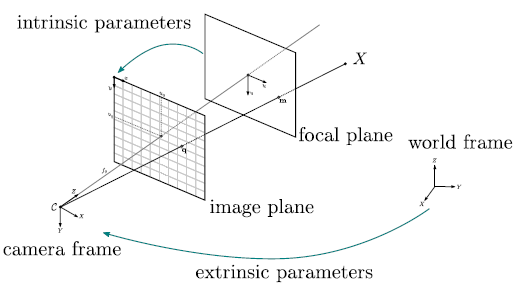
\includegraphics[width=0.7\linewidth]{chapters/camera/image3.png}
\caption{A pinhole-kameramodell.}
\label{fig:pinhole}
\end{figure}
	
	
A kamerához definiálható egy kamera koordináta-rendszer. Ennek a koordináta-rendszernek az origójában van a vetítés középpontja, a z tengelye merőleges a vetítés síkjára. A kép koordináta-rendszer síkbeli koordináta-rendszer, a síkra vetített pontokat értelmezzük ebben. $x$ és $y$ tengelyei a kamera koordináta-rendszer tengelyeivel egyirányúak, és általában $u$ és $v$ betűkkel jelöljük őket, megkülönböztetve őket a kamera koordináta rendszer tengelyeitől. Amennyiben homogén koordinátákkal jellemezzük a tér pontjait, mind a perspektív vetítés, mind a világ koordináta-rendszer és a kamera koordináta-rendszer közötti eltolás, forgatás mátrixszal kifejezhető: 

\begin{align}
\label{eq:cam-trf-basic}
&w \left[ \begin{array}{c} u \\ v \\ 1 \end{array} \right] = \mathbf{A} \; \mathbf{T} \left[ \begin{array}{c} x \\ y \\ z \\ 1 \end{array} \right] \\ \nonumber
&\mathbf{A} = 
\left[ 
\begin{array}{ccc}
f_x & \gamma & u_0 \\
0 & f_y & v_0 \\
0 & 0 & 1
\end{array}
\right] \\ \nonumber
&\mathbf{T} = \left[
\begin{array}{cc}
\mathbf{R} & \mathbf{t}
\end{array}
\right]
\end{align}

Ahol:
\begin{itemize}
\item $u\; v$ a képpont képi koordinátái. $w$ a homogén koordináták miatti komponens
\item $x,\; y,\; z$ a tárgypont koordinátái világ koordináta-rendszerben
\item $\mathbf{A}$ az úgynevezett kameramátrix
\item $f_x, \; f_y$ a kamera fókusztávolsága (ideális esetben egyenlőek, valós alkalmazásokban nem feltétlenül)
\item $\gamma$ egy \textit{skew} nevű torzítási paraméter, ami ideális esetben 0
\item $u_0,\; v_0$ a kamera principális pontjának koordinátái kép koordináta-rendszerben. Ez az a pont, ahol a kamera koordináta rendszer $z$ tengelye döfi a képsíkot
\item $\mathbf{T}$ a világ koordináta-rendszerből kamera koordináta-rendszerbe való transzformáció.
\item $\mathbf{R} \in \mathbb{R}^{3 \times 3}$ forgatási mátrix
\item $\mathbf{t} \in \mathbb{R}^{3 \times 1}$ eltolási vektor
\end{itemize}
 
A kameramátrix paramétereit kamera belső paramétereinek nevezzük. Mivel ezek a kamera rendeltetésszerű használata során nem változnak jelentősen, a kamera szerves részei, egyszeri kalibrálással meghatározhatók. A koordináta-rendszerek közti transzformáció paraméterei a külső paraméterek. Az összes paraméter meghatározható kellően nagy számú pontpár segítségével, ezt kamera-kalibrációnak nevezzük. Pontpárok alatt a világ koordináta-rendszerben ismert pozíciójú pontokat és azok kép koordináta-rendszerben megadott vetületét értjük. A tényleges kalibrációnál általában egy kalibráló objektumról több, különböző nézőpontból készült képet használunk. A kalibráló objektum jellemzően több, egyszerűen, de akár szubpixeles pontossággal detektálható pontból áll, például sakktábla-mintázat sarkai, vagy körökből álló rácsozat pontjainak közepe.

A valóságban a pinhole kameramodell sajnos nem állja meg a helyét, a képet többféle torzítás terheli például abból adódóan, hogy nem vetítést alkalmazunk, hanem lencserendszert, valamint, hogy a detektoron elhelyezkedő pixelek gyártástechnológiája nem tökéletes. Ezeket a paramétereket most nem mutatom be.

Az OpenCV-ben a kamera-kalibráció implementálva van, ami meghatározza mind a belső paramétereket, mind a torzítási paramétereket.

\section{Külső paraméterek meghatározása, PnP probléma}
%TODO módszerek leírása http://iplimage.com/blog/p3p-perspective-point-overview/

	A kamera használata során szükség van a külső paramétereinek ismeretére. Azt a feladatot, amely ismert térbeli helyzetű tárgypontok és a hozzájuk tartozó képi pontok alapján próbálja meghatározni a kamera külső paramétereit PnP, azaz Perspective-n-Point problémának nevezzük. 
	
Ennek egyik verziója a P3P algoritmus \cite{XiaoPnP}, amely csak 4 pontpárból számítja a paramétereket. Három pont kell ahhoz, hogy véges sok megoldást kapjunk (négy ponttal már túlhatározott lenne a feladat). A negyedik pontot az algoritmus arra használja fel, hogy a véges sok megoldás közül kiválassza a helyeset. Ezt úgy teszi meg, hogy a lehetséges négyféle megoldás közül azt választja, amelyikkel a negyedik pontot a képre vetítve a legkisebb hibát kapjuk a megadott képi ponthoz képest. Ezt aztán tetszőleges optimumkereséssel tovább lehet finomítani, pl. Levenberg-Marquardt eljárással. Ezt az eljárást használhatjuk akkor is, ha több, mint négy pont áll rendelkezése.

A PnP probléma megoldása során előfordulhat, hogy hibás pontpárosítások is kerülnek a bemeneti adatok közé. Többek között ennek a kiszűrésére alkalmas a következő szakaszban bemutatott algoritmus.

\section{RANSAC algoritmus}
A RANSAC (Random Sample Consensus) \cite{FischerRANSAC} algoritmus nem kifejezetten képfeldolgozási, hanem általános célú algoritmus, de az általam használt algoritmusok közül többnek részét képezi, ezért indokoltnak tartom bemutatni a működését. A RANSAC módszer annak a problémának egy megközelítése, amikor hibás mérésekkel terhelt adathalmazra próbálunk modellt illeszteni. Itt a modell lehet bármi, ami valamilyen pontossággal illeszkedik az adatokra. Ezt általában 2D ponthalmazra való egyenesillesztéssel szokás szemléltetni. A kiugró mérési hibák miatt jellemzően nem érdemes a legkisebb négyzetek módszerét használni, mert rossz illeszkedést fog mutatni. Ezt szemlélteti a következő ábra.

\begin{figure}[H]
\centering
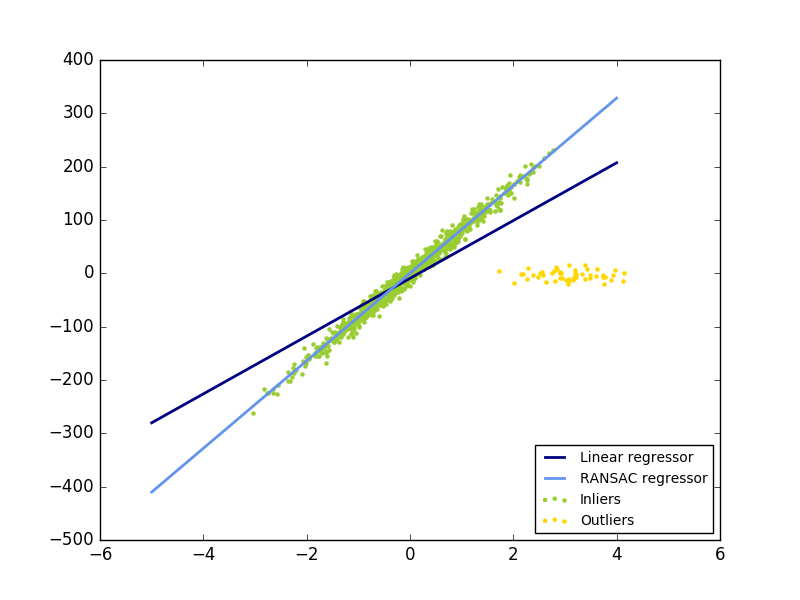
\includegraphics[width=0.7\linewidth]{chapters/camera/ransac.png}
%http://scikit-learn.org/stable/auto_examples/linear_model/plot_ransac.html
\caption{A RANSAC algoritmus és a legkisebb négyzetek módszerének összehasonlítása.}
\label{fig:ransac}
\end{figure}

Az algoritmus leírása során az angol terminológiát használom, a helyes mérési adatot \textit{inlier}-nek nevezem, a mérési hibát pedig \textit{outlier}-nek. 

A RANSAC algoritmus működése a következő:

\vspace{5mm}
\setlength\tabcolsep{0pt}
\noindent \begin{tabularx}{\textwidth}{rlllllllll}
%\noindent \begin{tabularx}{\textwidth}{|l|l|l|l|l|l|l|l|l|l|}
\hline
\multicolumn{10}{c}{\textbf{RANSAC algoritmus}} \\ \hline
1: \hspace{5pt} & \multicolumn{9}{l}{\textbf{eljárás} RANSAC($adatok$, $K$, $e$)} \\
2: \hspace{5pt} & \hspace{20pt} & \multicolumn{8}{l}{\textit{legjobb modell} $\leftarrow$ \textit{null}} \\
3: \hspace{5pt} & \hspace{20pt} & \multicolumn{8}{l}{\textbf{ciklus} $i \leftarrow 1,K$} \\
4: \hspace{5pt} & \hspace{20pt} & \hspace{20pt} & \multicolumn{7}{l}{\textit{vélt inlierek} $\leftarrow N$ darab véletlen adatpont} \\
5: \hspace{5pt} & \hspace{20pt} & \hspace{20pt} & \multicolumn{7}{l}{\textit{vélt modell} $\leftarrow$ \textit{vélt inlierek}-re illesztett modell} \\
6: \hspace{5pt} & \hspace{20pt} & \hspace{20pt} & \multicolumn{7}{l}{\textit{illeszkedők} $\leftarrow$ \textit{vélt modell}-re $e$ hibahatáron belül illeszkedő pontok} \\
7: \hspace{5pt} & \hspace{20pt} & \hspace{20pt} & \multicolumn{7}{l}{\textbf{ha} \textit{illeszkedők} száma $> N$} \\
8: \hspace{5pt} & \hspace{20pt} & \hspace{20pt} & \hspace{20pt} & \multicolumn{6}{l}{\textit{becsült modell} $\leftarrow$ \textit{illeszkedők}-re illesztett új modell} \\
9: \hspace{5pt} & \hspace{20pt} & \hspace{20pt} & \hspace{20pt} & \multicolumn{6}{l}{\textbf{ha} \textit{legjobb modell}-nél jobb \textit{becsült modell}} \\
10: \hspace{5pt} & \hspace{20pt} & \hspace{20pt} & \hspace{20pt} & \hspace{20pt} & \multicolumn{5}{l}{\textit{legjobb modell} $\leftarrow$ \textit{becsült modell}} \\
11: \hspace{5pt} & \hspace{20pt} & \multicolumn{8}{l}{\textbf{visszatérés} \textit{legjobb modell}\textbf{-lel}} \\
\hline
\end{tabularx}
\vspace{5mm}

Az algoritmus robusztussága abban rejlik, hogy ha a 4. sorban a \textit{vélt inlierek} közé nem kerül egyetlen outlier sem, a \textit{vélt modell}-re a legtöbb inlier illeszkedni fog $e$ hibahatáron belül, és a 8. sorban egy nagyon jó illeszkedésű modellt kapunk. Ebben az esetben akár le is lehet állítani az iterálást, és rögtön visszatérni a legjobb modellel.

A RANSAC algoritmus előnye, hogy nagy mennyiségű outlier jelenlétében is képes megtalálni az inlierekre illeszkedő modellt. Létezik olyan verziója is, amellyel 5\% inlier arány mellett is sikeres eredményeket értek el \cite{ransac5}. Hátránya, hogy a véletlenszerű működés miatt nem garantál "optimális" megoldást, és ha meg is találja, a végrehajtási idő véletlenszerűen változhat futásról futásra.

\chapter{Koordináta-rendszerek, Kéz-szem kalibráció}

A robotikában különböző koordináta-rendszereket használunk. Jelen feladat során a következő koordináta-rendszereket használom:
	\begin{itemize}
	\item A robot bázis koordináta-rendszere, avagy világ koordináta-rendszer. A robot nulladik, álló szegmenséhez van rögzítve. Betűjele: $R$ (Robot)	
	\item Megfogó vagy szerszám koordináta-rendszer, amely a robot utolsó szegmensének végén található. Betűjele: $T$ (Tool)
	\item Kamera koordináta-rendszer. Ennek a koordináta-rendszernek az origóját a pinhole modell alapján a vetítési pontba képzeljük el, a \textit{z} tengelye egybeesik az optikai tengellyel és a kamera nézési irányába mutat. A valóságban az optikai tengely és a lencse síkjának metszéspontjában található az origó. Betűjele: $C$ (Camera)
	\item Tárgy koordináta-rendszer. Ez az a koordináta-rendszer, amiben a megfigyelt tárgy pontjainak koordinátáit értelmezzük. Betűjele: $O$ (Object)
	\end{itemize}
	
	A $B$ koordináta-rendszerből az $A$ koordináta-rendszerbe való transzformáció a következőképpen írható fel homogén koordinátákban:
	
	\begin{equation}
	\label{eq:trf-kifejt}
	\mathbf{T}_{AB} = 
	\left[
	\def\arraystretch{1.2}
	\begin{array}{c|c}
 	\mathbf{R}_{AB} & \mathbf{t}_{AB} \\
 	\hline
	\mathbf{0}^T & 1 \\
	\end{array}	
	\right] \in \mathbb{R}^{4 \times 4}
	\end{equation}
	
	Itt $\mathbf{R}_{AB}$ 3x3-as rotációs mátrix, $\mathbf{t}_{AB}$ pedig oszlopvektor. A $\mathbf{t}_{AB}$ vektor az $A$ koordináta-rendszer origójából a $B$ koordináta-rendszer origójába mutat ($A$-ban felírva), míg $\mathbf{R}_{AB}$ oszlopai a $B$ koordináta-rendszer egységvektorai szintén $A$-ban felírva.
	
	A jelöléstechnikából következik, hogy ${\mathbf{T}_{AB}}^{-1} = \mathbf{T}_{BA}$

	A kéz-szem kalibráció során a robot megfogójának és a kamerának a relatív helyzetét kívánjuk meghatározni, azaz $\mathbf{T}_{TC}$-t (vagy inverzét). Amennyiben ez ismert, a kamera helyzetét képesek vagyunk világ koordináta-rendszerben is megadni, ugyanis a megfogó és a világ koordináta-rendszer közti transzformációt a direkt kinematikai probléma megoldásával meghatározhatjuk.

	A kalibrációhoz használt módszer a belső paraméterek kalibrálásánál alkalmazotthoz hasonló, egy kalibrációs objektumról képeket készítünk, amelyen megkeressük a tárgy ismert pozíciójú pontjait. Az így kapott összefüggésekből számítjuk először a kamera külső paramétereit, majd az egyéb ismert paraméterek felhasználásával a kamera relatív helyzetét.	
	
	A fent ismertetett koordináta-rendszerek közötti transzformációs lánc felírható:
	
	\begin{equation}\label{eq:trf-lanc1}
	\mathbf{T}_{CO}\mathbf{T}_{OR}\mathbf{T}_{RT}\mathbf{T}_{TC} = \mathbf{I}
	\end{equation}
	
	Az egyes transzformációknak speciális tulajdonságaik vannak, amit kalibráláskor ki lehet (sőt kell) használni. A kamera a végberendezésre szilárdan van rögzítve, nem mozdul el. A robot is rögzítve van a gépalaphoz, amihez képest a kalibráló tárgy nem mozog a kalibráció során. Ez azt jelenti, hogy a $\mathbf{T}_{OR}$ és $\mathbf{T}_{TC}$ mátrixok nem változnak, ha a robotkart mozgatjuk. Ezen felül ismert a robotkar pozíciója a bázis koordináta-rendszerben, hiszen megkaphatjuk a direkt geometriai feladat megoldásával. A PnP algoritmus továbbá megadja a kamera helyzetét a tárgy koordináta-rendszerben. Így $\mathbf{T}_{CO}$ és $\mathbf{T}_{RT}$ mátrixok ismertek minden kép esetében.
	
	A kalibráció két lépésben történik. Az első lépésben a rotációs mátrixokat számítjuk ki, a másodikban a transzlációs vektorokat.
	
	Először azonban a kalibrációhoz szükséges Kabsch algoritmus működését mutatom be.
	
	\section{Kabsch algoritmus}	

	A Kabsch algoritmus \cite{Kabsch} két vektorhalmaz közti optimális forgatási mátrixot számítja ki. A probléma felvetése a következő. Adottak ${\mathbf{p}_i}^T \in \mathbb{R}^{1 \times 3}$ és ${\mathbf{q}_i}^T \in \mathbb{R}^{1 \times 3}$ vektorok, $i=1..N$. Keressük azt az $\hat{\mathbf{R}} \in \mathbb{R}^{3 \times 3}$ mátrixot, amelyre:
	
\begin{equation}
\hat{\mathbf{R}} = \underset{\mathbf{R}}{ arg\,min} \; \sum_{i=1}^N \left\lVert\mathbf{p}_i	- \mathbf{R} \mathbf{q}_i\right\rVert^2
\end{equation}
	
	Az algoritmus a vektorhalmazok közti koordinátánkénti kovariancia-mátrixot számítja ki, majd ennek SVD felbontásából határozza meg az optimális forgatást:
	
	\begin{equation}
	\label{eq:kabsch-bigmat}
	\mathbf{P} \coloneqq \left[ \begin{matrix}
		\vdots \\
		{\mathbf{t}_{RTi}}^T \\
		\vdots
		\end{matrix} \right] \in \mathbb{R}^{N \times 3} , \quad
	\mathbf{Q} \coloneqq \left[ \begin{matrix}
		\vdots \\
		{\mathbf{t}_{OCi}}^T \\
		\vdots
		\end{matrix} \right] \in \mathbb{R}^{N \times 3} , \quad
		i = 1..N
	\end{equation}
	\begin{equation}
	\mathbf{A} = \mathbf{P}^T\mathbf{Q}
	\end{equation}
	\begin{equation}
	\mathbf{U \Sigma V}^T = \mathbf{A}
	\end{equation}
	\begin{equation}
	\hat{\mathbf{R}} = \mathbf{U}\left[
\begin{matrix}
1 & 0 & 0 \\
0 & 1 & 0 \\
0 & 0 & det(\mathbf{UV}^T) \\
\end{matrix}
	 \right]\mathbf{V}^T
	\end{equation}
	
	Érdemes megjegyezni, hogy a vektorhalmazok tömegközéppontja az origóban kell hogy legyen, amennyiben ez nem teljesül, könnyen korrigálható a vektorok eltolásával.
	
	\section{A rotációk becslése}
	A \eqref{eq:trf-lanc1} egyenletet átalakítva kapjuk, hogy:
	
	\begin{equation}
	\label{eq:trf-lanc2}
	\mathbf{T}_{OC} = \mathbf{T}_{OR}\mathbf{T}_{RT}\mathbf{T}_{TC}
	\end{equation}
	
	Ha az egész egyenletet beszorozzuk jobbról a nullvektorral:
	
	\begin{equation}
	\mathbf{T}_{OC}\left[ \begin{array}{c} 0 \\ 0 \\ 0 \\ 1 \end{array}	 \right] = \mathbf{T}_{OR}\mathbf{T}_{RT}\mathbf{T}_{TC}\left[ \begin{array}{c} 0 \\ 0 \\ 0 \\ 1 \end{array}	\right]
	\end{equation}	
		
	És elvégezzük a megfelelő szorzásokat, kapjuk:
	
	\begin{equation}
	\left[
	\begin{array}{c}
		\mathbf{t}_{OC}\\
		1
	\end{array}
	\right]	
	 = \mathbf{T}_{OR} 
	 \left[
	\begin{array}{c}
	\mathbf{R}_{RT}\mathbf{t}_{TC} + \mathbf{t}_{RT} \\ 1
	\end{array}	
	 \right]
	\end{equation}
	
	Ebben az egyenletben számunkra ismeretlen a $\mathbf{T}_{OR}$ mátrix és a $\mathbf{t}_{TC}$ vektor. A kalibráció során készítünk $N$ darab képet, amelyekhez meghatározzuk a külső paramétereket, vagyis a $\mathbf{T}_{OC}$ mátrixot. Ezeket a képeket úgy készítjük el, hogy az $\mathbf{R}_{RT}$ mátrix állandó, vagyis két kép készítése között nem forgatjuk a kamerát, csak eltoljuk. Ekkor kiegészíthető a fenti egyenlet egy, a kép sorszámát jelölő indexszel:
	
	\begin{equation}
	\label{eq:rot-est}
	\left[
	\begin{array}{c}
		\mathbf{v}_{OCi}\\
		1
	\end{array}
	\right]	
	 = \mathbf{T}_{OR} 
	 \left[
	\begin{array}{c}
	\mathbf{R}_{RT}\mathbf{t}_{TC} + \mathbf{t}_{RTi} \\ 1
	\end{array}	
	 \right] \quad i = 1..N
	\end{equation}
	
	Azok az ismeretlenek, illetve paraméterek, amik nem kaptak indexet, azok állandóak a képek készítése során. Vegyük a fenti $N$ darab egyenlet átlagát:
	
	\begin{equation}
	\label{eq:rot-est-avg}
	\left[
	\begin{array}{c}
	 	\frac{\sum \mathbf{t}_{OCi}}{N}\\
		1
	\end{array}
	\right]	
	 = \mathbf{T}_{OR} 
	 \left[
	\begin{array}{c}
	\mathbf{R}_{RT}\mathbf{t}_{TC} + \frac{\sum \mathbf{t}_{RTi}}{N} \\ 1
	\end{array}	
	 \right]
	\end{equation}	
	
	Ha kivonjuk a \eqref{eq:rot-est-avg} egyenletet a \eqref{eq:rot-est} egyenletből, a következőt kapjuk:
		
	\begin{equation}
	\label{eq:rot-trf1}
	\left[
	\begin{array}{c}
	 	\mathbf{t}_{OCi} - \frac{\sum \mathbf{t}_{OCi}}{N}\\
		0
	\end{array}
	\right]	
	 = \mathbf{T}_{OR} 
	 \left[
	\begin{array}{c}
	\mathbf{t}_{RTi} - \frac{\sum \mathbf{t}_{RTi}}{N} \\ 0
	\end{array}	
	 \right]
	\end{equation}	
	
	Bevezetjük, hogy:
	
	\begin{equation*}
	\begin{split}
	 	\overline{\mathbf{t}_{OCi}} &\coloneqq \mathbf{t}_{OCi} - \frac{\sum \mathbf{t}_{OCi}}{N} \\
	 	\overline{\mathbf{t}_{RTi}} &\coloneqq \mathbf{t}_{RTi} - \frac{\sum \mathbf{t}_{RTi}}{N} 
	 	\end{split}
	\end{equation*}
	
	Szemléletesen a felülvont változó az adott vektornak az összes vektor tömegközéppontjához képesti relatív helyzetét mutatja meg. Vegyük észre, hogy ezek kiszámíthatók, ismerjük őket. \eqref{eq:rot-trf1} írható a következő alakban is:
	
	\begin{equation}
	\left[
	\begin{array}{c}
	 	\overline{\mathbf{t}_{OCi}}\\
		0
	\end{array}
	\right]	
	 = \left[
	\def\arraystretch{1.2}
	\begin{array}{c|c}
 	\mathbf{R}_{OR} & \mathbf{t}_{OR} \\
 	\hline
	\mathbf{0}^T & 1 
	\end{array}	
	\right]
	 \left[
	\begin{array}{c}
	\overline{\mathbf{t}_{RTi}} \\ 0
	\end{array}	
	 \right]
	\end{equation}
	
	Ebből pedig:
	
	\begin{equation}
 	\overline{\mathbf{t}_{OCi}}	= \mathbf{R}_{OR} 	\overline{\mathbf{t}_{RTi}}
	\end{equation}
	
	$\mathbf{R}_{OR}$ kiszámítása tehát ekvivalens az kapott vektorpárok közti optimális rotáció kiszámításával, amit Kabsch algoritmus számít ki.
	
	Ez után $\mathbf{R}_{TC}$ számítása történik. \eqref{eq:trf-lanc1} alapján: 
	
	\begin{equation}
	\mathbf{R}_{TRi}\mathbf{R}_{RO}\mathbf{R}_{OCi} = \mathbf{R}_{TCi}\quad i = 1 .. N
	\end{equation}
	
	A jobb oldalon található rotációs mátrixok "átlagát" kellene venni, ezt is a Kabsch algoritmussal lehet kiszámítani. Az algoritmusnak azonban vektorpárokra van szüksége, nem pedig mátrixokra. Ebben az esetben $3N$ darab vektorpár alapján végezzük a számítást, minden átlagolandó rotációhoz 3-3 vektorpár tartozik: egy ilyen párhármas egyik tagja a rotációs mátrix megfelelő oszlopvektora, a másik tagja pedig a neki megfelelő egységvektor ($\left[1\:0\:0 \right]^T $, $\left[0\: 1\: 0 \right]^T $, vagy $\left[0\: 0\: 1 \right]^T $). Ekkor a \eqref{eq:kabsch-bigmat}-ben definiált mátrixok a következő alakot öltik:
	
	\begin{equation}
	\mathbf{P} \coloneqq \left[ \begin{matrix}
		\vdots \\
		\mathbf{R}_{TCi} \\
		\vdots
		\end{matrix} \right], \quad
	\mathbf{Q} \coloneqq \left[ \begin{matrix}
		\vdots \\
		\mathbf{I} \\
		\vdots
		\end{matrix} \right], \quad
		i = 1..N
	\end{equation}
	
	ahol $\mathbf{I}$ a $3\times 3$-as egységmátrix.
	
	Így a rotációk átlagát véve a Kabsch algoritmussal megkaphatjuk az $\mathbf{R}_{TC}$ mátrixot.
	
	\section{A transzlációk becslése}
	Ha kifejtjük a \eqref{eq:trf-lanc2} egyenletet \eqref{eq:trf-kifejt} szerint, kapjuk, hogy:
	
	\begin{equation}
	\left[ 	\def\arraystretch{1.2} \begin{array}{c|c}
 	\mathbf{R}_{OC} & \mathbf{t}_{OC} \\ \hline
	\mathbf{0}^T & 1 \\
	\end{array}	\right] = 	
	\left[ \def\arraystretch{1.2} \begin{array}{c|c}
 	\mathbf{R}_{OR} & \mathbf{t}_{OR} \\ \hline
	\mathbf{0}^T & 1 \\
	\end{array}	\right]	
	\left[ \def\arraystretch{1.2} \begin{array}{c|c}
 	\mathbf{R}_{RT} & \mathbf{t}_{RT} \\ \hline
	\mathbf{0}^T & 1 \\
	\end{array}	\right]	
	\left[ \def\arraystretch{1.2} \begin{array}{c|c}
 	\mathbf{R}_{TC} & \mathbf{t}_{TC} \\ \hline
	\mathbf{0}^T & 1 \\
	\end{array}	\right]
	\end{equation}
	
	Összeszorozva a jobb oldalt a következő adódik:
	
	\begin{equation}	
	\left[ \def\arraystretch{1.2} \begin{array}{c|c}
 	\mathbf{R}_{OC} & \mathbf{t}_{OC} \\ \hline
	\mathbf{0}^T & 1 \\
	\end{array}	\right] = 
	\left[ \def\arraystretch{1.2} \begin{array}{c|c}
 	\mathbf{R}_{OR}\mathbf{R}_{RT}\mathbf{R}_{TC} & \mathbf{R}_{OR}\mathbf{R}_{RT}\mathbf{t}_{TC}+\mathbf{R}_{OR}\mathbf{t}_{RT} + \mathbf{t}_{OR} \\ \hline
	\mathbf{0}^T & 1 \\
	\end{array}	\right]
	\end{equation}
	
	Az ebben a fázisban elkészített képek számát jelöljük $M$-mel. Ebből, ha bevezetjük az indexet a változó paraméterekhez , kapjuk, hogy:
	
	\begin{equation}
	\mathbf{t}_{OCi} = \mathbf{R}_{OR}\mathbf{R}_{RTi}\mathbf{t}_{TC}+\mathbf{R}_{OR}\mathbf{t}_{RTi} + \mathbf{t}_{OR} \quad i=1..M
	\end{equation}
	
	Vegyük észre, hogy most már a megfogó orientációját, azaz az $\mathbf{R}_{RTi}$ mátrixot is változtatjuk a képek készítése során. A fenti egyenletben a $\mathbf{t}_{TC}$ és $\mathbf{t}_{OR}$ vektorok az ismeretlenek. Átrendezve az egyenletet:
	
	\begin{equation}
	{\mathbf{R}_{OR}}^{-1} \mathbf{t}_{OCi} -  \mathbf{t}_{RTi} =  \mathbf{R}_{RTi}\mathbf{t}_{TC}+{\mathbf{R}_{OR}}^{-1}\mathbf{t}_{OR}
	\end{equation}
	
	Bevezetve:
	
	\begin{equation}
	\begin{split}
	\mathbf{p}_i &\coloneqq {\mathbf{R}_{OR}}^{-1} \mathbf{t}_{OCi} -  \mathbf{t}_{RTi} \\
	\mathbf{A}_i &\coloneqq  \mathbf{R}_{RTi} \\
	\mathbf{B} &\coloneqq  {\mathbf{R}_{OR}}^{-1}
	\end{split}
	\end{equation}
	
	Kapjuk, hogy:
	
	\begin{equation}
	\mathbf{p}_i =  \mathbf{A}_i\mathbf{t}_{TC}+\mathbf{B}\mathbf{t}_{OR}
	\end{equation}
	
	Ha az összes $M$ egyenletet egybefoglaljuk:
	
	\begin{equation}
	\mathbf{Cx} = \mathbf{k}
	\end{equation}
	
	ahol:
	
	\begin{equation}
	\mathbf{x} \coloneqq \left[ \begin{matrix} \mathbf{t}_{TC} \\ \mathbf{t}_{OR}\end{matrix}	 \right], \quad
	\mathbf{C} \coloneqq  \left[ \begin{array}{cc} \multicolumn{2}{c}{\vdots} \\ \mathbf{A}_i & \mathbf{B} \\ \multicolumn{2}{c}{\vdots}  \end{array} \right], \quad
	\mathbf{k} \coloneqq  \left[ \begin{matrix} \vdots \\ \mathbf{p}_i \\ \vdots \end{matrix} \right] 
	\end{equation}
	\begin{equation*}
	\mathbf{x} \in \mathbb{R}^{6 \times 1}, \quad
	\mathbf{C} \in \mathbb{R}^{3M \times 6}, \quad
	\mathbf{k} \in \mathbb{R}^{3M \times 1}, \quad
	i = 1..M
	\end{equation*}
	
	Innen a pszeudoinverz segítségével az optimális megoldás számolható:
	
	\begin{equation}
	\hat{\mathbf{x}} = \left(\mathbf{C}^T \mathbf{C}\right)^{-1}\mathbf{C}^T\mathbf{k}
	\end{equation}
\chapter{Kulcspontkeresés és -párosítás}
\section{Kulcspontkereső algoritmusok}
	
	A kulcspontkereső algoritmusok célja olyan pontok megtalálása a képen, amelyek valamely környezete vizuálisan érdekes, jól elkülöníthető, egyedi. Céljuk továbbá, hogy ezekhez a pontokhoz olyan jellemző mennyiséget rendeljenek, amely alapján az adott pont egy másik képen is megtalálható. Ennek a mennyiségnek minél inkább függetlennek kell lennie a kép készítésének minél több körülményétől. A mennyiséggel szemben támasztott követelmény tehát, hogy legyen invariáns a képalkotáskor előforduló minél többféle transzformációra, mint például a skálázás, az elforgatás, vagy a fényerő változása. A jellemző mennyiség a legtöbb algoritmus esetében egy tulajdonság-leíró vektor, vagy leíróvektor, röviden csak leíró.
	
	\subsection{SIFT kulcspontkeresés}
	
	A SIFT (Scale Invariant Feature Transform) \cite{LoweSIFT} egy kulcspontkereső algoritmus. Az általa generált leíró egy 128-elemű vektor, amely invariáns eltolásra, elforgatásra, skálázásra, a megvilágítás kismértékű megváltozására, zajra, és a kamera pozíciójának kismértékű megváltozására. Nem invariáns a projektív transzformációra, tehát a kamera helyzetének jelentős megváltozására.
	
	Az algoritmus főbb lépései a következők:
	
	\begin{enumerate}
	\item Kulcspont-jelöltek skálainvariáns detektálása
	\item Szubpixeles lokalizáció
	\item Kulcspont-jelöltek szűrése
	\item Jellemző orientáció meghatározása
	\item Lokális orientáció-hisztogramok számítása
	\item Leíró-generálás
	\end{enumerate}
	
	\subsubsection{Kulcspont-jelöltek skálainvariáns detektálása}
	Az algoritmus első lépéseként a képen érdekesnek tűnő pontokat keresünk. Ezt DoG (Difference of Gaussians) szűrőkkel érjük el. A DoG szűrő a képet különböző mértékű (szórású) Gauss-szűrésnek veti alá, majd ezek különbségét veszi. Így az élkiemeléshez hasonló képet kapunk, ám legjobban a szórás méretébe eső térfrekvenciájú részletek kerülnek kiemelésre. A szűrést különböző szórású kernelekkel elvégezve különböző mérettartományokba eső képrészleteket emelhetünk ki. Az így megtalált szélsőértékeket tekintjük kulcspont-jelöltnek.
	
	\subsubsection{Szubpixeles lokalizáció}
	A kulcspontok szubpixeles lokalizációjához az egyes dimenziókban (x, y, skála) másodfokú közelítést alkalmazunk, és így keressük meg a valódi szélsőérték helyét pixel alatti és skálafaktornál nagyobb pontossággal.
	
	\subsubsection{Kulcspont-jelöltek szűrése}
	Az algoritmus eddig a lépésig sok olyan pontot is megjelölt, amelynek képi helyzete nem egyértelmű, pl. egy homogén régiót, vagy élt jellemeznek a képen, nem pedig egy pontot. Ezek kerülnek kiszűrésre ebben a lépésben. A szűrés során az adott pontban kiszámoljuk a másodfokú deriváltakból álló Hesse-mátrixot. Ennek a mátrixnak a sajátértékei szolgálnak információval a pont környezetéről. Amennyiben mindkét sajátérték kicsi, a pont környezete homogén. Ha az egyik kicsi, a másik pedig nagy, élszerű pontról beszélhetünk. A "kicsi" és "nagy" fogalmak természetesen kvalitatívak, a számszerű értékek tapasztalati úton kerülnek meghatározásra, az algoritmus paraméterei. Ezeket az élszerű és homogén környezetű pontokat ebben a lépésben eldobjuk.
	
	\subsubsection{Jellemző orientáció meghatározása}
	Az orientációhoz hisztogramot használunk, amelynek 36 osztálya van, mindegyik 10°-ot fed le. A kulcspont környezetében minden pontban kiszámítjuk a gradiensvektort, majd ennek irányának megfelelően a hisztogram adott osztályába tesszük. A maximális orientációt másodfokú interpolációnak alávetve határozzuk meg a jellemző orientációt. Amennyiben több kiugróan gyakori orientáció van a hisztogramban, a kulcspontot lemásoljuk, és mindegyik jellemző orientációval újat hozunk létre. Így érjük el az elforgatás-invarianciát.
	
	\subsubsection{Lokális orientáció-hisztogramok számítása}
	A képpont 16x16 pixeles környezetét felosztjuk 4x4 darab 4x4-es blokkra. Minden blokkhoz létrehozunk egy 8-osztályos orientáció-hisztogramot, amibe az adott pixeleknek az előző lépésben meghatározott orientációhoz képesti relatív gradiens-iránya kerül.
	
	\subsubsection{Leíró-generálás}
	A leíró-vektor elemeit az előző lépésben kiszámolt hisztogram osztályainak gyakoriságai adják. A 4x4 darab 8-osztályos hisztogramból így 128-elemű vektort kapunk. Ezt a vektort megvilágítás-invariancia céljából normalizáljuk.
	
	\subsection{SURF kulcspont-keresés}
	A SURF (Speeded Up Robust Features) \cite{HerbertSURF} algoritmus hasonló elven működik, mint a SIFT, ám az egyes lépésekhez különböző megoldásokat alkalmaz. A kulcspont-jelöltek keresésénél a Gauss-szűrést ún. box-filterrel közelíti, amit az integrális képből számol. Az integrális kép $(x,y)$ koordinátájú pixelének intenzitását az alábbi összefüggés adja:
	
\begin{equation}
S(x, y) = \sum_{i=0}^x \sum_{j=0}^y I(i, j)
\end{equation}

Ahol $S(x, y)$ az integrális kép intenzitása az $(x, y)$ pontban, $I(i, j)$ pedig az eredeti kép intenzitása az $(i, j)$ pontban.
	
	Az integrális kép tehát azon pixelek összegét tartalmazza, amelyek egy megadott téglalapon belül találhatók. E téglalap bal felső sarka a kép bal felső sarkával esik egybe, a jobb alsó pedig az $(x,y)$ pixel. Az integrális kép használatának előnye, hogy egy adott téglalapon belüli pixelek összegzését nagyon meggyorsítja, amire mind a box-filterhez, mind a Hesse-mátrix közelítéséhez szükség van.
	
	Az algoritmus azokat fogja érdekes pontoknak venni, ahol a Hesse-mátrix determinánsa lokálisan maximális. A pontosság érdekében itt is interpoláljuk a megoldást. Az orientáció meghatározásnál egy adott Euklideszi norma szerinti (kör alakú) környezeten belül található pontok (Haar-wavelet válaszával közelített) gradiens-irányát veszi figyelembe, és egy csúszóablakkal történő kereséssel határozza meg a domináns orientációt. A leíró-generálásnál a kulcspont környezetét 4x4-es blokkokra osztja, és ezekhez a blokkokhoz rendel egy négyelemű vektort, amit a gradiensek alapján számít. Így 4x4x4, azaz 64-elemű leíróvektort kapunk.
	
	\section{Leíró-párosító algoritmusok, párosítás-szűrések}
	\label{matching}
	A kulcspontdetektáló algoritmus megkereste a képen az érdekes pontokat, leíró-vektort generált hozzájuk. Ezt két különböző képen elvégezve az így kapott leírókat párosítanunk kell, ha megfeleltetéseket akarunk találni a kulcspontok között. Mivel a leírók n-dimenziós vektorok, ezért két leíró közötti hasonlóságot egyszerűen lehet számszerűsíteni, pl. a különbségük L2 normájával. A probléma abból adódik, hogy nagyméretű képeken sok (1000-es nagyságrendű) leírónk van, és ezeket kell másik, hasonló méretű leíró-halmazhoz párosítani.
	
	A legegyszerűbb megoldás a brute force módszer, vagyis mindegyiket mindegyikkel összehasonlítjuk. Ez lassú ugyan, de garantáltan a legjobb megoldást adja. Egy másik megoldás a FLANN (Fast Library for Approximate Nearest Neighbors) algoritmus \cite{muja_flann_2009}, ami gyors, de csak közelítő megoldást ad.
	
	Az algoritmusok garantáltan sok hibás párosítást is eredményeznek, ezeket feltétlenül szűrni kell, amelyekre több módszer is van, a következőkben ezeket mutatom be. Mindegyik algoritmus bemutatása során egy $d$ vektorhoz keresünk párt a $B$ halmazból, ahol $d$ egy leíróvektor az egyik képen megtaláltak közül, $B$ pedig a másik képen megtalált leírók halmaza. Az alábbiakban a \cite{OpenCV}-ben található, valamint az epipoláris egyenesekkel történő szűréseket mutatom be.
	
	\subsection{Arányteszt alapú párosítás-szűrés}
	Ez a heurisztikus módszer azon a feltételezésen alapul, hogy a helyes párosítás esetén $d$ sokkal közelebb van a párjához, mint más vektorokhoz. Hamis párosításnál azonban semmi nem indokolja, hogy a legjobb párosítás lényegesen jobb legyen a többinél, mondjuk a második legjobbnál.
	
	Éppen ezért ez a szűrés azokat a párosításokat tartja meg, amelyeknél a legjobb megtalált $B$-beli vektor ($b_{best}$) és a második legjobb vektor ($b_{best2}$) közötti távolságok aránya nagy:
	\begin{equation}
	\frac{\|d-b_{best}\|}{\|d-b_{best2}\|}\ll 1
	\end{equation}
	
	A gyakorlatban az aránynak a küszöbértékét $0,6..0,8$ közé szokás választani.
	
	\subsection{Keresztellenőrzéses szűrés}
	\label{match-cross}
	Ez a módszer azt a feltételezést használja, hogy ha $d$ és $e$ pontok párok a két képen, akkor nincs olyan más vektor $e$-n kívül az ő halmazában, ami $d$-hez közelebb lenne, viszont $e$-hez sem találni $d$-nél közelebb lévő vektort. Ez a szűrés akkor fogadja el a párt, ha kölcsönösen a legközelebb helyezkednek el egymáshoz.
	
	\subsection{Epipoláris egyenes használata}
	\label{match-epilines}
	Amennyiben ismerjük a két képhez tartozó kamerapozíciót, az első képen megtalált összes ponthoz definiálható a második képen egy síkbeli egyenes, amely egyenes mentén a pont párja elhelyezkedhet. Ezt hívjuk epipoláris egyenesnek. Ennek az információnak a birtokában a párosításnál vehetjük eleve csak az epipoláris egyenesre illeszkedő pontokat, és azokhoz párosítjuk a $d$ leírót, vagy a párosítás után eldobhatjuk azokat a párokat, ahol a megtalált kulcspont nem illeszkedik az egyenesre, így kevesebb párt kapunk majd, viszont gyorsabb a számítás.
	
	\subsection{Homográfia-alapú szűrés}
	\label{match-homogr}
	A homográfia megfeleltetés két kép pontjai között. Amennyiben a képek egy sík tárgyról (pl. könyvborítóról) készültek és egy adott tárgypontnak a képi koordinátái ismertek az egyik képen, a homográfia segítségével meghatározhatók ugyanannak a tárgypontnak a képi koordinátái a másik képen is. 
	A homográfia meghatározható véges sok pontpár segítségével. A hibás párosításokat RANSAC algoritmussal kiszűrhetjük, amikor a párosításokra homográfiát illesztünk, így az algoritmus nagy mennyiségű hibás adat esetén is jól működik.
	A módszer hátránya, hogy csak sík objektumokra használható.
\chapter{3D rekonstrukció}

	A 3D rekonstrukció során egy térbeli objektum pontjainak koordinátáit kívánjuk meghatározni. Ez sok esetben különböző nézőpontból készült képek alapján történik. A problémát megoldó algoritmusokat a szakirodalomban \textit{Structure from Motion (SfM)}, vagy \textit{Multi-View Stereo (MVS)} algoritmusoknak hívják. Amennyiben a kamera külső paraméterei ismertek, a probléma lineáris legkisebb négyzetek módszerével megoldható. A külső paraméterek hiányában a feladat nemlineáris legkisebb négyzetek problémává alakítható, amelyet célszerű Levenberg-Marquardt algoritmussal megoldani. Ennek a nemlineáris problémának a megoldását \textit{bundle adjustment}-nek hívják.
	
	A 3D rekonstrukció kimenete általában egy pontfelhő. Amennyiben csak kulcspontok párosítását használjuk, és azok térbeli helyzetét határozzuk meg, ún. ritka pontfelhőt kapunk. Ha teljes 3D-s modellt akarunk kapni, vagyis a teljes megfigyelt környezetet vissza akarjuk állítani, akkor sűrű pontfelhőre van szükségünk. Jelen alkalmazásban a ritka pontfelhő elegendő.
	 
\section{Többnézetes háromszögelés}	 	
\label{muli-view-triang} 
	Mivel számunkra ismertek a kamera külső (és belső) paraméterei, ezért a feladat egy (túlhatározott) lineáris egyenletrendszer megoldása. A probléma precíz megfogalmazása a következő: Adott egy ismeretlen helyzetű 3D-s tárgypont, amelyről $N$ darab képet készítettünk ismert térbeli helyzetből. A tárgypontnak megfelelő képi pontokat az összes képen ismerjük. Keressük azt a 3D-s pontot, amelyet a kamerák képsíkjaira visszavetítve az ismert képi pontoktól való távolságok négyzetösszege minimális.
	
	A \eqref{eq:cam-trf-basic} egyenlet alapján írható:
	
	\begin{equation}
	\label{eq:mvs-trf-basic}
	w_i \left[ \begin{array}{c} u_i \\ v_i \\ 1 \end{array} \right] = \mathbf{P}_i \left[ \begin{array}{c} x \\ y \\ z \\ 1 \end{array} \right] , \quad \mathbf{P}_i \in \mathbb{R}^{3 \times 4}, \quad i = 1..N
	\end{equation}
	
	Az \eqref{eq:mvs-trf-basic} egyenlet minden képre felírható, ismertek $\mathbf{P}_i$, $u_i$, $v_i$, és keressük $x$, $y$ és $z$ értékét. Ha bevezetjük, hogy:
	
	\begin{equation}
	\mathbf{P}_i \eqqcolon \left[ \begin{array}{cc} 
	\mathbf{p}_{1i} & a_{1i} \\
	\mathbf{p}_{2i} & a_{2i} \\
	\mathbf{p}_{3i} & a_{3i} \\
	 \end{array} \right], \quad 
	 \mathbf{p}_{1i}, \,
	 \mathbf{p}_{2i}, \, 
	 \mathbf{p}_{3i} \in \mathbb{R}^{1 \times 3}
	\end{equation}
	
	valamint:
	
	\begin{equation}
	\mathbf{x} \coloneqq \left[ \begin{array}{ccc} x & y & z \end{array} \right]^T
	\end{equation}
	
	Az \eqref{eq:mvs-trf-basic} egyenlet írható a következő formában:
	
	\begin{equation}
	\begin{split}
	w_i u_i &= \mathbf{p}_{1i}\mathbf{x} + a_{1i} \\
	w_i v_i &= \mathbf{p}_{2i}\mathbf{x} + a_{2i} \\
	w_i &= \mathbf{p}_{3i}\mathbf{x} + a_{3i}
	\end{split}
	\end{equation}
	
	A fenti két egyenletbe az alsót behelyettesítve adódik:
	
	\begin{equation}
	\begin{split}
	\left(\mathbf{p}_{3i}\mathbf{x} + a_{3i}\right)u_i &= \mathbf{p}_{1i}\mathbf{x} + a_{1i} \\
	\left(\mathbf{p}_{3i}\mathbf{x} + a_{3i}\right)v_i &= \mathbf{p}_{2i}\mathbf{x} + a_{2i}
	\end{split}
	\end{equation}
	
	Ezt az egyenletet $\mathbf{x}$-rendezve és az összes képre felírva kapjuk, hogy:
	
	\begin{equation}
	\mathbf{G}\mathbf{x}=\mathbf{b}
	\end{equation}
	
	ahol:
	
	\begin{equation}
	\mathbf{G} \coloneqq \left[
	 \begin{array}{c}
	 	\vdots \\ 
	 	\mathbf{p}_{3i}u_i - \mathbf{p}_{1i} \\ 
	 	\mathbf{p}_{3i}v_i - \mathbf{p}_{2i} \\
	 	\vdots
	\end{array}	 \right], 
	\quad \mathbf{b} \coloneqq \left[ 
	\begin{array}{c}
		\vdots \\
		a_{1i} - a_{3i} u_i \\ 
		a_{2i} - a_{3i} v_i \\
		\vdots
\end{array}	 \right]
	\end{equation}
	
	Innen a pszeudoinverz segítségével számolható az optimális megoldás:
	
	\begin{equation}
	\hat{\mathbf{x}} = \left(\mathbf{G}^T\mathbf{G}\right)^{-1}\mathbf{G}^T\mathbf{b}
	\end{equation}
	
	Fontos megjegyezni, hogy ez a megoldás nem a visszavetítési hibát minimalizálja, hanem az egyenletrendszer algebrai hibáját ($\hat{\mathbf{Gx}-b}$ mennyiséget). Amennyiben ez lényeges eltérést okoz, nemlineáris optimumkereséssel meghatározható a valódi optimum. Ezt az implementáció során elhanyagoltam.

	\section{Leíró-párosító algoritmusok sajátosságaiból adódó problémák}
	A feladat bonyolultsága fokozható, ha figyelembe vesszük, hogy a párosító algoritmusok téves párosításokat is tartalmaznak, valamint, hogy egy leíróhoz lehet, hogy csak kevés (egy vagy kettő) másikat sikerül párosítani még több kép esetén is. Minél több párt talál a párosító algoritmus egy leíróhoz, annál pontosabban határozható meg a hozzá tartozó kulcspont 3D pozíciója.
	
	A párosításokat értelmezhetjük ritka, nem összefüggő gráfként, ahol a csúcsok a kulcspontok és azok leírói, az élek pedig a párosításokat jelentik. Értelemszerűen ha feltételezzük, hogy minden párosítás helyes, akkor minden összefüggő részgráf egy-egy tárgyponthoz tartozó leírókat tartalmaz. 
	
	A tesztek alapján, amiket végeztem, azt lehet mondani, hogy 5 tesztkép esetén mindegyiket mindegyikkel párosítva a csomópontok több, mint feléből csak egyetlen él fut ki, azaz a hozzájuk tartozó leírókhoz a többi 4 képből csak egyen sikerült párt találni. A tesztek azt támasztják tehát alá, hogy a gráf kellően ritka.
	
\subsection{A ritkaság korrigálása}	
	\label{extension_doc}
	
	A gráf sűrítése érdekében megtehetjük azt, hogy pl vesszük az összes olyan csúcs-hármast, amelyik majdnem teljes részgráfot (kvázi-klikket) alkot, vagyis a 3 élből csak egy hiányzik, és teljessé tesszük, bízva abban, hogy a párosító algoritmus valamilyen oknál fogva a behúzott élnek megfelelő párosítást nem találta helyesnek, pedig az. Ezt megtehetjük bármilyen csúcs-$n$-esre is.
	
\subsection{Téves párosítások szűrése}

	A téves párosítások figyelembe vételéhez érdemes RANSAC elven működő algoritmust alkalmazni. Ekkor a meghatározandó modell a 3D pozíció lesz. A 3D pozíciót visszavetítve a képekre az illeszkedés mértékét definiálhatjuk az így kapott képi pontok és az eredetileg detektált pontok közti négyzetes távolságösszegként.
\chapter{Megvalósítás}
\section{A szoftver feladatai}
A konkrét implementáció a BME IIT robotlaborjában történt egy Mitsubishi robotkaron. A komplett, több komponensből álló szoftver feladatai a következők:

\begin{itemize}
\item A robotkar mozgatása a PC-n bevitt helyzetbe.
\item A kéz-szem kalibráció automatikus elvégzése.
\item A 3D rekonstrukció elvégzése.
\item A tárgy helyzetének meghatározása 3D pontfelhőt tartalmazó adatbázis alapján.
\end{itemize}	

\section{Kiválasztott implementáció}
A tárgy helyzetének meghatározásához készítünk egy képet a tárgyról. Ezen a képen kulcspontkeresést hajtunk végre, majd párosítjuk ezeket a pontokat a 3D pontfelhő pontjaival. A pozíció és orientáció becslése PnP algoritmussal történik.

Az előző fejezetekben a legtöbb probléma megoldására több módszert is ismertettem. Itt szeretném bemutatni az implementációhoz kiválasztottakat.

\subsection{Kulcspontkeresés és -párosítás implementációja}
A kulcspontkeresés SURF algoritmussal történik. 

A párosító algoritmus minden esetben a \ref{matching} szakaszban ismertetett brute force párosító, mivel az több párosítást eredményez, mint a FLANN algoritmus. 

A 3D rekonstrukció során a kulcspontpárosításnál ismerjük a külső paramétereket, ezért a \ref{match-epilines} és \ref{match-homogr} szakaszokban ismertetett, epipoláris egyeneseket és homográfiát használó szűrést alkalmazom. A homográfiás szűrés esetén RANSAC elvű algoritmust használok.

Mivel a tárgy pozíciójának becslésekor épp a külső paramétereket kívánjuk meghatározni, ezért itt az epipoláris egyenesek használata nem lehetséges. Ennél a lépésnél a \ref{match-cross} szakaszban ismertetett keresztellenőrzéses szűrést alkalmazom.

\subsection{A kéz-szem kalibráció implementációja}

A kéz-szem kalibrációnál különböző nézőpontokból képeket kell készíteni egy kalibráló objektumról. Először az orientáció megtartásával, majd annak változtatásával. Sajnos a megvalósításhoz használt robotkar munkatere nem túl nagy, valamint a kamera látószöge is elég kicsi, ezért a kamera helyzetét nem lehet széles tartományban változtatni. Ez a kéz-szem kalibráció esetében az első fázisban (állandó orientáció) $\pm 5$ cm-es tartományt jelent mindhárom tengely mentén. Így a program 11 képet készít mind az $x$, $y$ és $z$ tengely mentén. A második fázisban a kalibráló objektum közepét a kép közepén tartva különböző szögekből készít képeket az algoritmus. Az $x$ tengely körül $\pm 15°$ elfordulást képes megvalósítani, az $y$ tengely körül a $\left[-9°, +30°\right]$ tartományban lehet változtatni az orientációt. Mindkét irányban szintén 11-11 képet készít a program.

A kalibráló objektum egy sakktáblamintázat volt, amit a \ref{fig:reconstr-img} ábrán is láthatunk. A minta sarokpontjainak meghatározásához az OpenCV-ben kész függvény van megírva, ezért ez nagyban megkönnyíti a kalibráció implementálását.

\subsection{3D rekonstrukció és a kéz-szem kalibráció implementációja}

A 3D rekonstrukció során a megtalált kulcspontpárok alapján a program egyszerű háromszögeléssel számít 3D pozíciót. A többnézetes háromszögelés módszerét végül elvetettem. 

Ahogy a kéz-szem kalibrációnál, úgy a 3D rekonstrukciónál is különböző nézőpontból kell képeket készíteni. Itt azonban a rekonstruálandó tárgyról készülnek a képek. Itt is probléma a limitált munkatér. A megvalósítás során az egyik tengely mentén $\left[-10°, +30°\right]$, a másik mentén pedig $\pm 30°$ tartományban készít a program képeket a tárgyról. A képek középpontjában ugyanúgy a tárgy "középpontját" tartja, viszont a két tengely körüli elforgatást egymástól függetlenül hajtja végre. Mindkét irányban 7 pontra osztottam fel az elfordulást, így összesen 49 kép készül a tárgyról. A külső paraméterek meghatározásához PnP algoritmust használ a program. Ugyanazt a sakktáblamintát használom, mint a kalibráció során.

\begin{figure}[H]
\centering
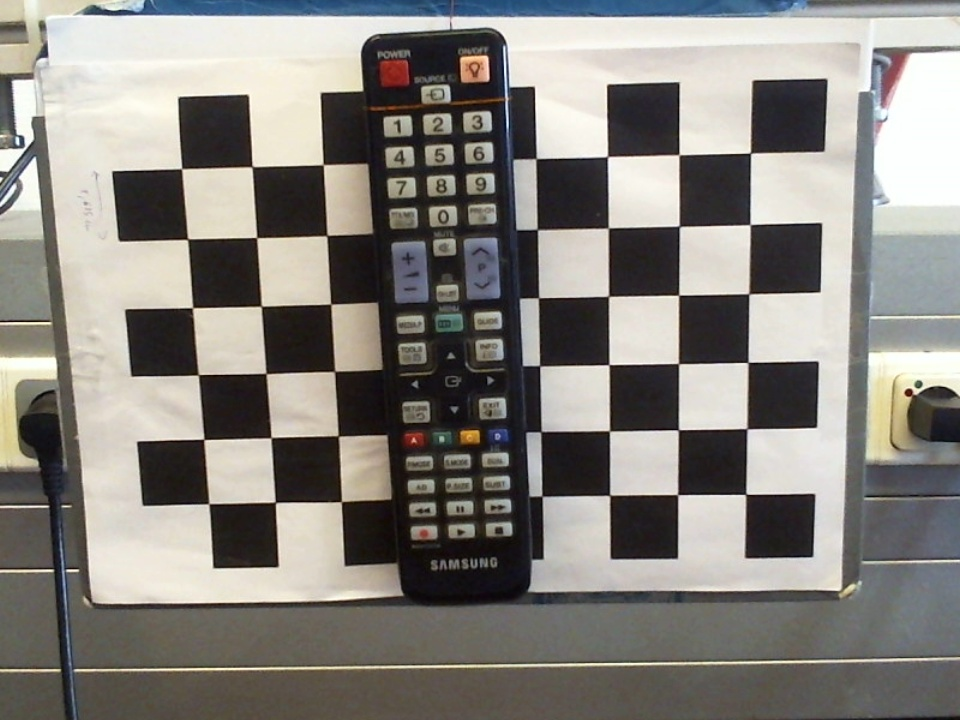
\includegraphics[width=\linewidth]{chapters/implementation/3dreconstr.jpg}
\caption{A rekonstrukcióhoz használt elrendezés. A rekonstruálandó tárgy egy TV-távirányító.}
\label{fig:reconstr-img}
\end{figure}

\subsection{A pozíció és orientáció meghatározásának implementációja}

A pozíció és orientáció meghatározása a PnP algoritmus RANSAC elvű megvalósításával történik. Amennyiben ismerjük a kamera pozícióját a tárgy koordináta-rendszerében, a \eqref{eq:trf-lanc1} egyenlet alapján kiszámolhatjuk a tárgy és a robot koordináta-rendszerek közti transzformációt, $\mathbf{T}_{OR}$-t. Ennek az ismeretében pedig a tárgyhoz képesti tetszőleges célkonfigurációba irányíthatjuk a robotkart.

A tárgy pozíciójának meghatározásához a szoftver öt különböző nézőpontból készít képeket. Mindegyikhez megpróbálja meghatározni a kamera külső paramétereit, és végül a mellett a konfiguráció mellett dönt, amelyet a legtöbb inlier alapján sikerül meghatározni. Ez után kiszámítja azt a konfigurációt, amelyben a kamera egyenesen ránéz a \ref{fig:cel-konf-cam} ábrán bekarikázott gombra, és majdnem érinti a távkapcsolót , ahogy az a \ref{fig:megfog-konf} ábrán látszik. Ez a megfogási konfiguráció. A program azonban (lehetséges ütközéseket elkerülendő) a megfogási konfigurációhoz képest egy eltolt célkonfigurációba irányítja a robotot. A célkonfiguráció a világ koordináta-rendszerben pozitív $z$ irányban (fölfele) 20 cm-rel van eltolva a megfogási konfigurációhoz képest. Ezt a \ref{fig:cel-konf} ábrán látjuk.

\begin{figure}[H]
\centering     %%% not \center
\subfigure[Megfogási konfiguráció]{\label{fig:megfog-konf}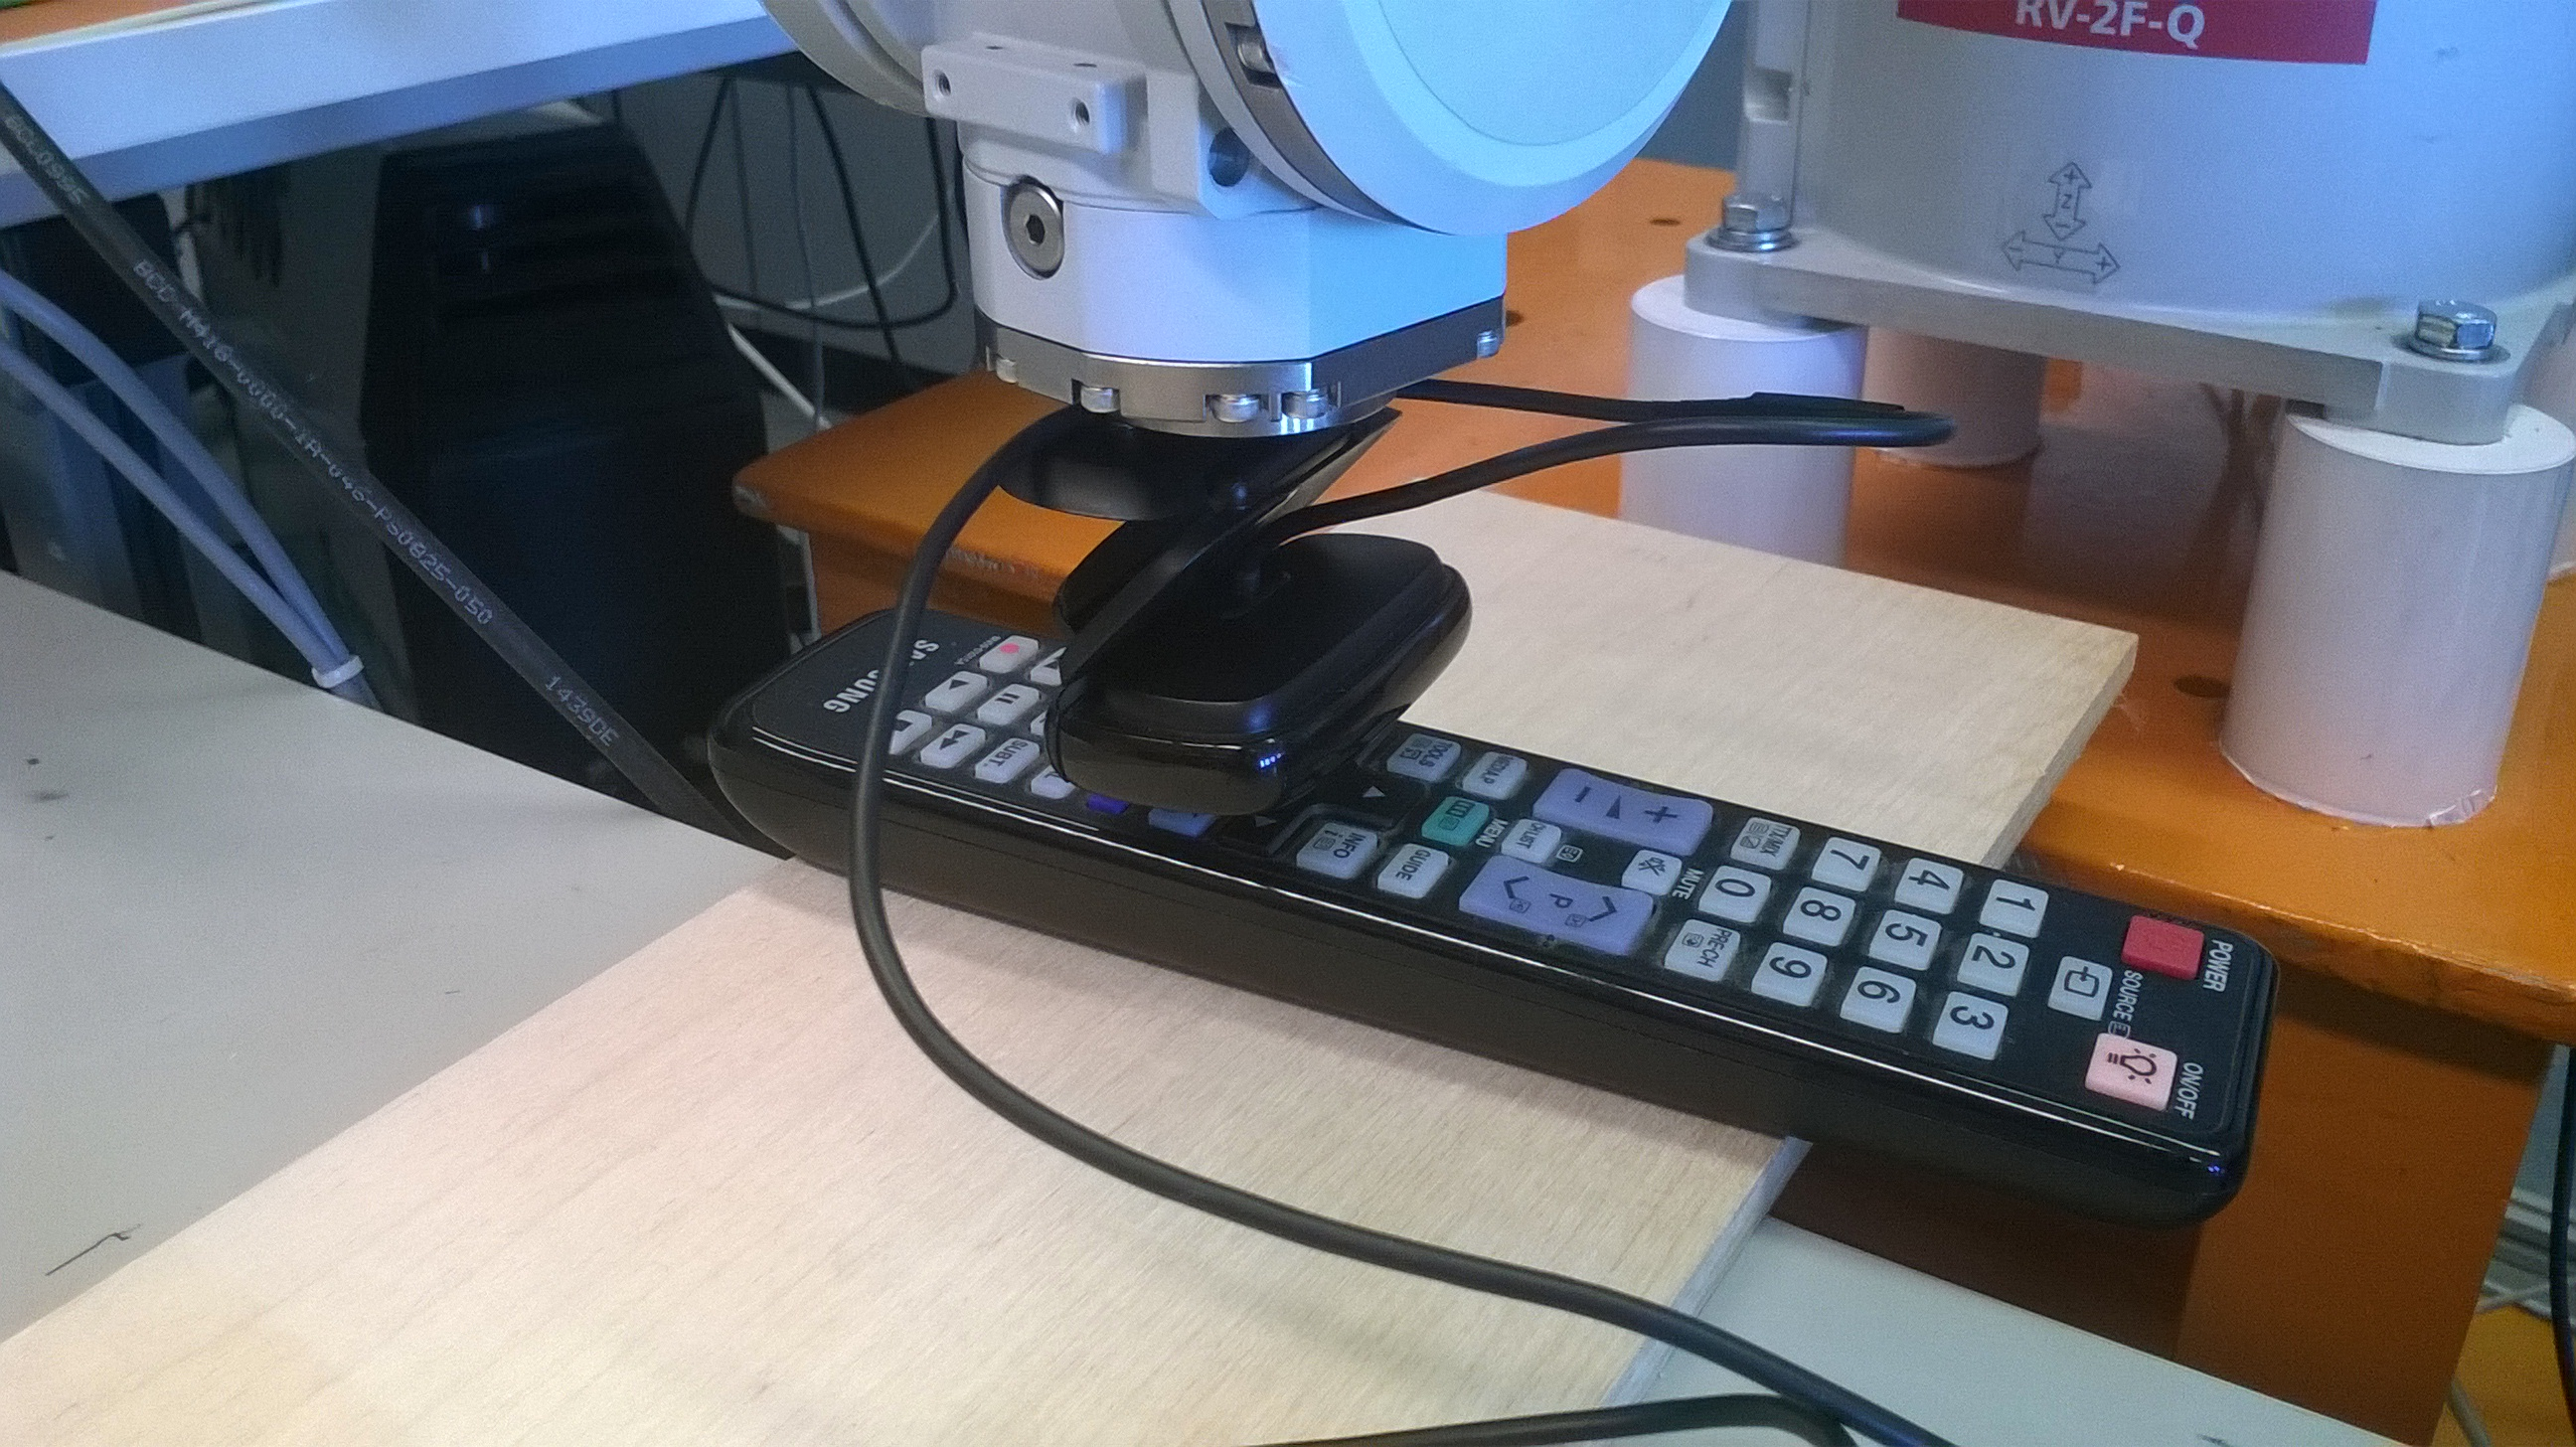
\includegraphics[width=0.45\linewidth]{chapters/implementation/megfog.jpg}}
\subfigure[Célkonfiguráció]{\label{fig:cel-konf}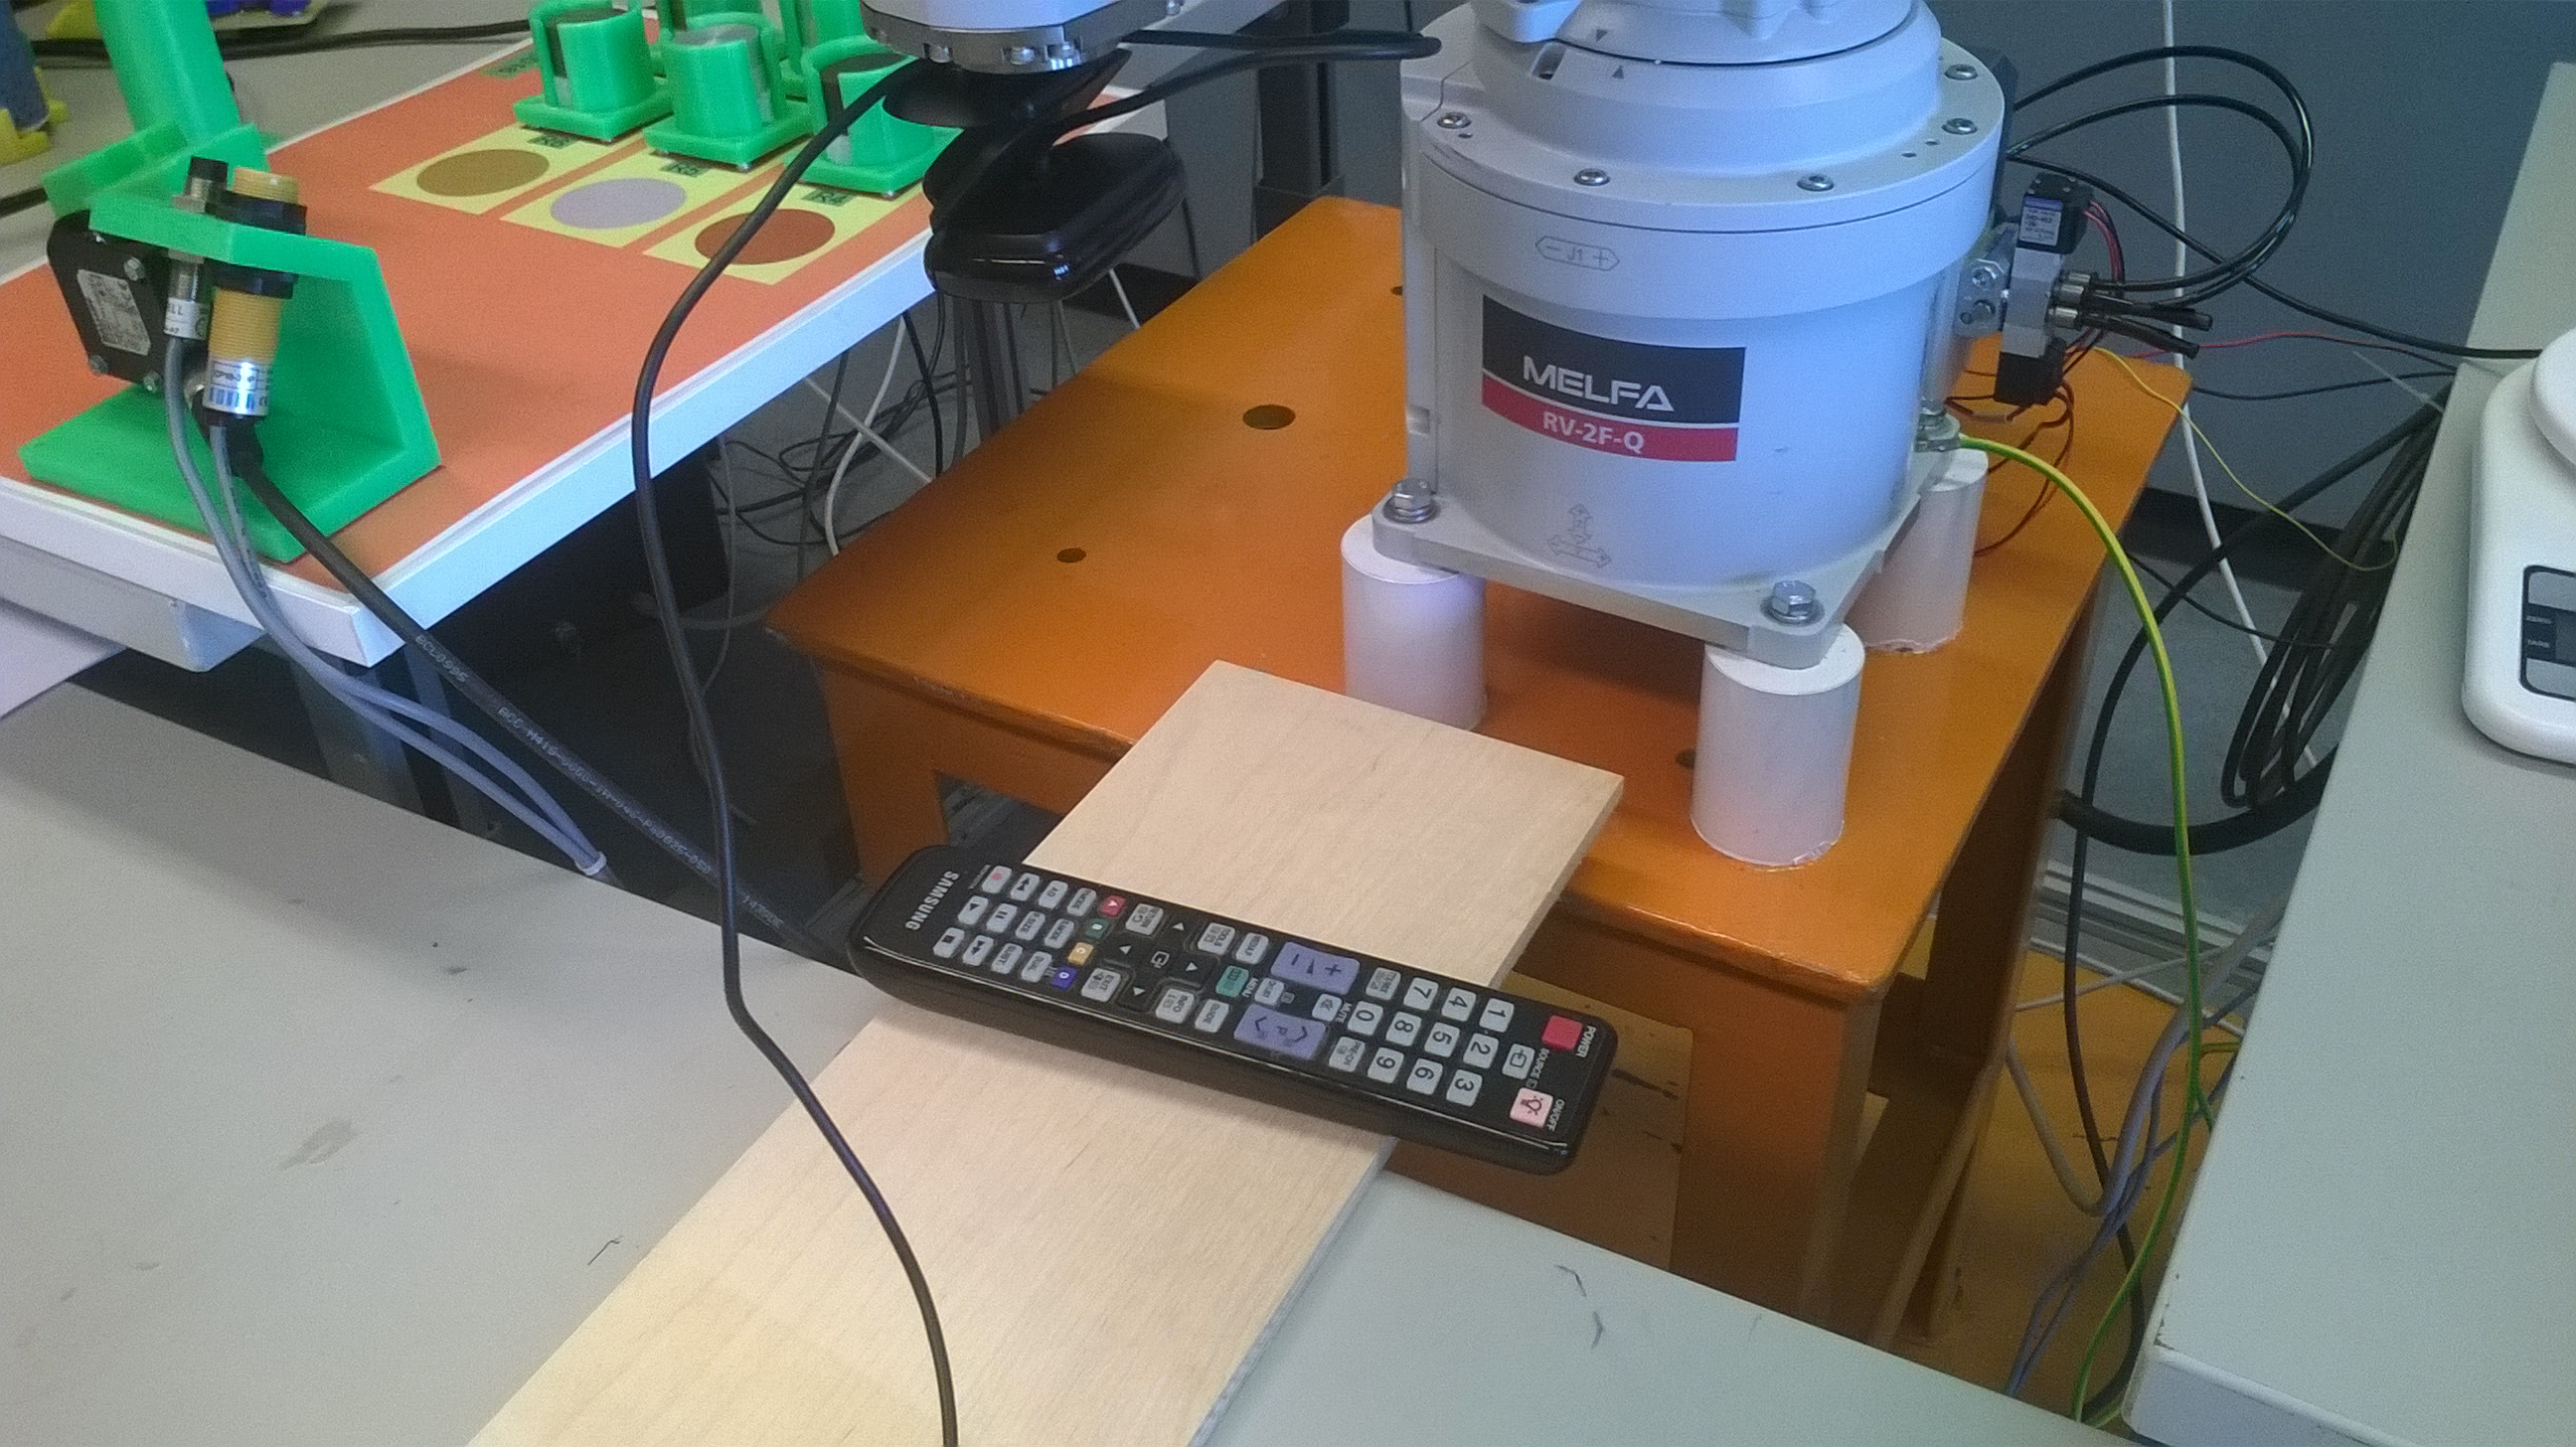
\includegraphics[width=0.45\linewidth]{chapters/implementation/cel.jpg}}
\subfigure[A kamera képe a célkonfigurációban.]{\label{fig:cel-konf-cam}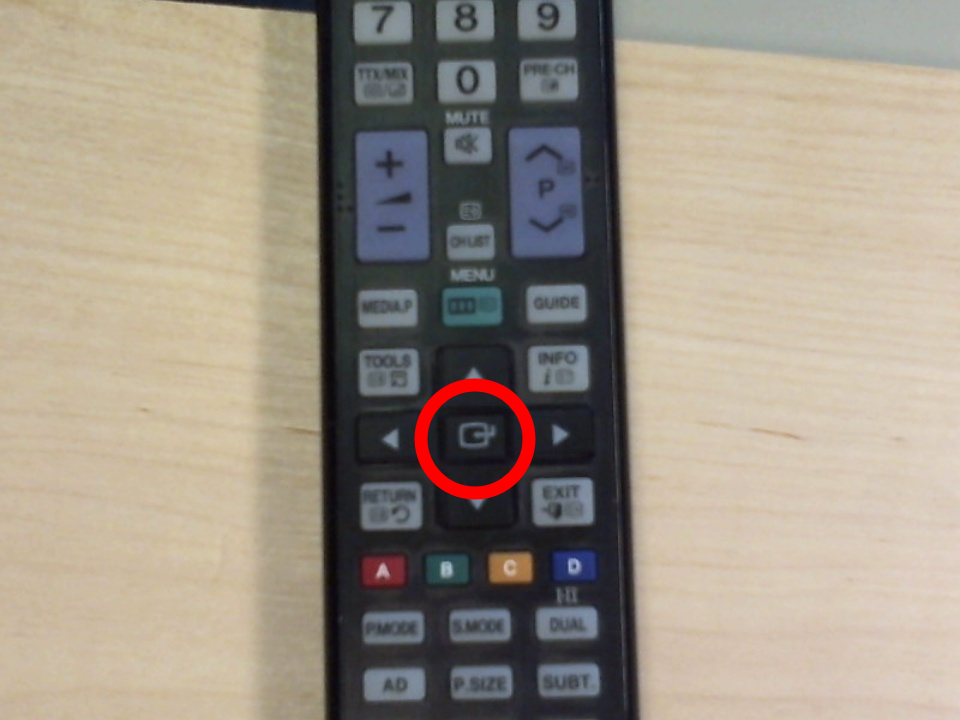
\includegraphics[width=0.45\linewidth]{chapters/implementation/cel_cam.png}}
\caption{A célkonfiguráció meghatározása}
\end{figure}

\section{A robotirányító rendszer felépítése}
	A komplett rendszer hardverkomponensei között lévő kommunikációs lánc a következő elemekből épül fel:
	
\begin{enumerate}
\item PC
\item PLC (Q03UDVCPU)
\item Robotvezérlő modul (Q172DRCPU)
\item Robotkar (Melfa RV-2F-Q)
\end{enumerate}	

	A kommunikáció a következő módon valósul meg. A PC és PLC között a kommunikáció Modbus/TCP kapcsolaton keresztül történik, a PLC a belső hálózaton DHCP-vel kiosztott statikus IP-n elérhető. A Modbus/TCP egy Ethernet-alapú kommunikációs protokoll, amelyben a szerver elérhetővé teszi a hozzá csatlakozott kliensek számára a regisztereit, azok szabadon írhatók, olvashatók. A PLC és a robotvezérlő modul megosztott memórián keresztül kommunikálnak. A robotvezérlő közvetlenül irányítja a robotkart, azzal egy komplett berendezést alkot, a köztük lévő kommunikáció megoldása nem a felhasználó feladata.
	
\begin{figure}[H]
\centering
\includegraphics[width=\linewidth]{chapters/implementation/system.png}
\caption{A robotirányító rendszer felépítése.}
\end{figure}
	
	A robot megfogójára egy Logitech c525 típusú webkamera van szerelve, ez szolgáltatja a képfeldolgozás számára a vizuális információt.
	
	
\begin{figure}[H]
\centering
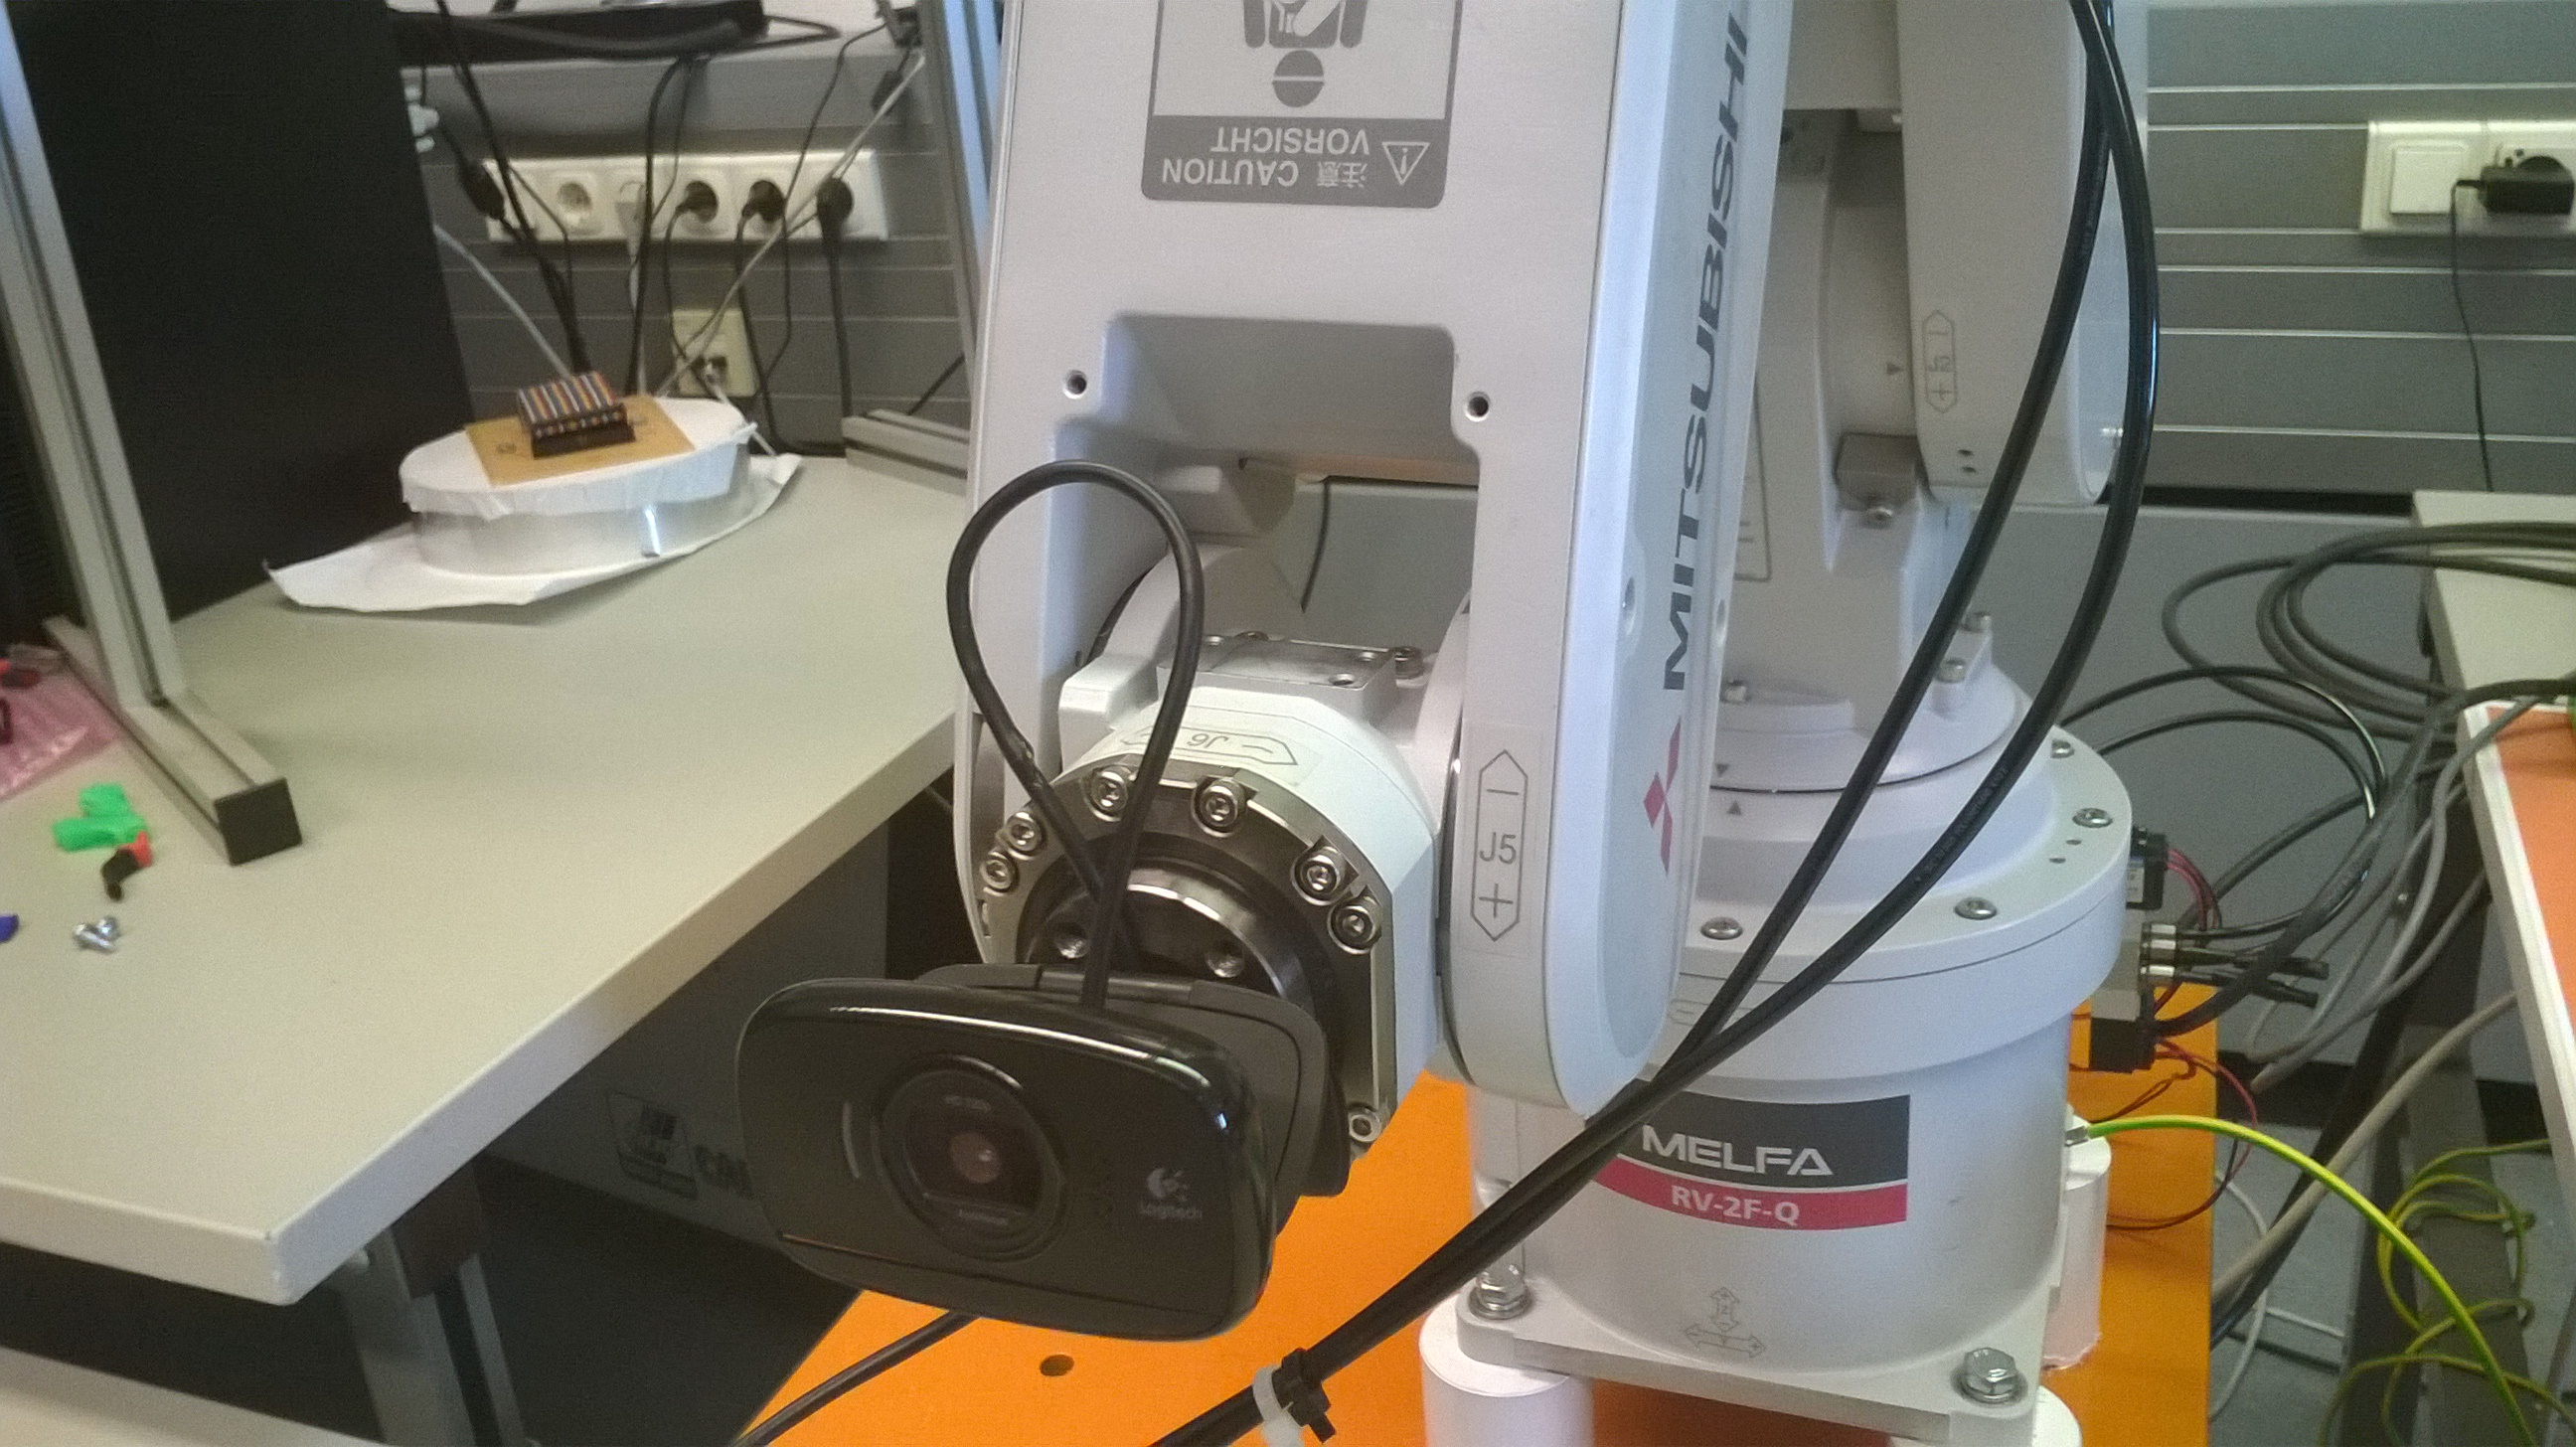
\includegraphics[width=\linewidth]{chapters/implementation/robocam.jpg}
\caption{A robotra szerelt kamera.}
\end{figure}
	
	\section{A PLC és robotprogram}
	
	A PLC-n két, a működéshez szükséges program fut. Az egyik egy Modbus szerver, ami a PC-vel való kommunikációt kezeli. Ez a Mitsubishi cég (és a programot korábban felfedező és használó hallgatók) jóvoltából már rendelkezésre állt számomra. 
	
	A másik program a robot felé történő kommunikációért felelős. Minthogy a PLC csak összekötő szerepet játszik a robot és a PC között, ezért ennek a programnak a feladatköre arra korlátozódik, hogy a Modbus-on keresztül kapott értékeket továbbítsa a megosztott memóriába. Ezt a programot Menyhárt Balázs MSc hallgató készítette, én minimális módosításokkal az ő programját használom.
	
	A roboton futó program kiolvassa a megosztott memóriából a megfelelő értékeket, és ennek megfelelően mozgatja a robotkart. Ennek a megvalósítása úgy történik, hogy egy-egy regiszterben kerül átadásra a pozíció-orientáció 6 paramétere. A robotprogram elvégzi a megfelelő korrekciókat (szög-radián átváltás), majd a megadott helyzetbe irányítja a megfogót. Ez ki van még egészítve egy utasításszámlálóval, amelynek értékét a PC-n futó programban vizsgálva megtudhatjuk, hogy az adott utasítást a robot elvégezte-e már.

	\section{A PC program}
	
	A PC programot Python nyelven írtam. Képfeldolgozásra az OpenCV függvénykönyvtárat, a Modbus kommunikáció megvalósításához a PyModbusTCP könyvtárat használtam.

	Csatlakozás után a megadott helyzetbe lehet irányítani a robotot, illetve a megfelelő gomb megnyomásával a kéz-szem kalibráció és a tárgy megkeresése is elvégezhető.
	
\begin{figure}[H]
\centering
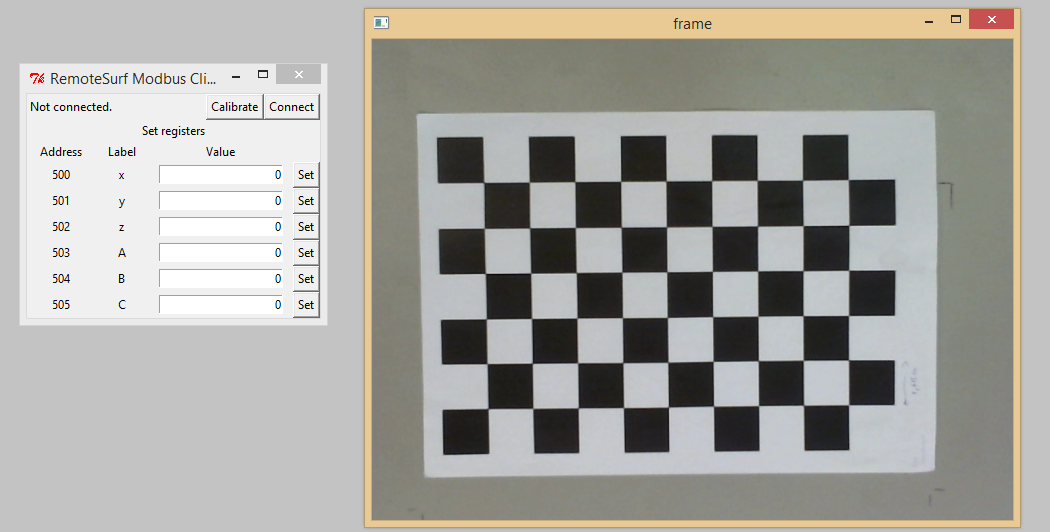
\includegraphics[width=\linewidth]{chapters/implementation/gui.png}
\caption{A program felhasználói felülete.}
\label{img-gui}
\end{figure}

	A legtöbb általam használt algoritmus OpenCV-s implementációját használom. Saját implementációk közül a legfontosabb a kéz-szem kalibráció algoritmusa és az \ref{muli-view-triang} fejezetben ismertetett háromszögelés algoritmusa. 
		
	A Kabsch algoritmust implementáló kódrészt Jimmy Charnley Kromann és Lars Andersen Bratholm írta, az ő kódjukat használom \cite{kabschGithub}.
	
\chapter{Eredmények}

A szoftver teszteléséhez a megtalálandó tárgy a \ref{fig:reconstr-img} ábrán látható TV-távirányító volt. A választás azért esett erre a tárgyra, mert kellően részletgazdag, és a mérete megfelelő a teszteléshez.

%A tárgy pozíciójának meghatározásához a szoftver öt különböző nézőpontból készít képeket. Mindegyikhez megpróbálja meghatározni a kamera külső paramétereit, és végül a mellett a konfiguráció mellett dönt, amelyet a legtöbb inlier alapján sikerül meghatározni. Ez után kiszámítja azt a konfigurációt, amelyben a kamera egyenesen ránéz arra a gombra, amely a távirányító négy nyílbillentyűje között található. Ez lenne a megfogási pozíció. A program azonban (lehetséges ütközéseket elkerülendő) a megfogási konfigurációhoz képest egy eltolt célkonfigurációba irányítja a robotot. A célkonfiguráció a világ koordináta-rendszerben pozitív $z$ irányban (fölfele) 20 cm-rel van eltolva a megfogási konfigurációhoz képest.
%
%%TODO képek megfogási- és célkonfigurációról

A tárgy pozíciójának meghatározását több elrendezésre is elvégeztem, elrendezésenként többször is lefuttatva a keresést. itt három ilyen teszt eredményét mutatom be, a tesztek során a keresést rendre 7, 7 és 6 alkalommal futtattam le. A megfogási konfiguráció ideális értékét kézzel állítottam be, ehhez képest mértem az ideális célkonfigurációt.

A három elrendezés a következő volt:

%TODO képek az elrendezésekről

%A, B, C elrendezés

Az eredmények közlésénél a következő jelölést használom:

\begin{itemize}
\item $\delta_x$, $\delta_y$, $\delta_z$, $\delta$ a két végpont közötti koordinátánkénti és abszolút különbség. $\delta^2=\delta_x^2+\delta_y^2+\delta_z^2$
\item $\Delta_x$, $\Delta_y$, $\Delta_z$, $\Delta$ rendre a két orientáció $x$, $y$ és $z$ tengelyei által bezárt szög és ezek számtani közepe. Amennyiben az orientációk megegyeznek, ezek természetesen nullával egyenlők.
\end{itemize}

% bevezetek egy mértéket, amely két orientáció különbözőségét méri. A helyes és a kapott orientáció eltérése úgy kerül számításra, hogy az orientációk által definiált bázisvektorok által bezárt szögek abszolút értékének vesszük az átlagát:
%
%\begin{equation}
%\Delta_{rot}(\mathbf{A}, \mathbf{B}) \coloneqq \frac{\angle (\mathbf{a}_1,\mathbf{b}_1) + \angle (\mathbf{a}_2,\mathbf{b}_2) + \angle (\mathbf{a}_3,\mathbf{b}_3)}{3} = \frac{\tr \left(\arccos\left(\mathbf{A}^T\mathbf{B}\right)\right)}{3}
%\end{equation}
%
%Ahol:
%
%\begin{equation*}
%\begin{split}
%\mathbf{A} &= \left[ \begin{array}{ccc} \mathbf{a}_1 & \mathbf{a}_2 & \mathbf{a}_3 \end{array} \right] \in \mathbb{R}^{3\times 3}, \quad \mathbf{A}^{-1} = \mathbf{A}^T \\
%\mathbf{B} &= \left[ \begin{array}{ccc} \mathbf{b}_1 & \mathbf{b}_2 & \mathbf{b}_3 \end{array} \right] \in \mathbb{R}^{3\times 3}, \quad \mathbf{B}^{-1} = \mathbf{B}^T
%\end{split}
%\end{equation*}
%
%A definícióból szemléletesen adódnak a következő tulajdonságok:
%
%\begin{itemize}
%\item $\Delta_{rot}(\mathbf{A}, \mathbf{A}) = 0$
%\item $\Delta_{rot}(\mathbf{A}, \mathbf{-A}) = \pi$
%\item $0 \leq \Delta_{rot}(\mathbf{A}, \mathbf{B}) \leq \pi$
%\end{itemize}

Az eredményeket a következő táblázatok mutatják.

%x, y, z trans eltérések, trans eltérés (gyök(négyzetösszeg)), x, y, z tengely szögeltérés, rot eltérés, inlierek sz. (trans cm-ben, rot fokban)
%data1
%[ 4.23  1.07  2.1 ], 4.84, [ 32.24  21.74  28.28], 27.42, 189
%[ 0.46 -1.5   4.63], 4.89, [ 21.62  21.62   0.4 ], 14.55, 157
%[ 0.81  0.02  4.08], 4.16, [ 6.6   5.96  2.99], 5.18, 76
%[ 4.32  1.06  1.97], 4.86, [ 32.58  22.76  27.9 ], 27.75, 183
%[-0.15 -0.64 -1.61], 1.74, [ 44.05  16.33  41.91], 34.10, 130
%[-0.38 -0.3  -1.91], 1.97, [ 32.07   3.97  31.89], 22.65, 152
%[ 0.33  0.07  2.25], 2.27, [ 10.13   0.37  10.14], 6.88, 101
%data2
%[ 1.76 -0.58 -5.35], 5.66, [ 46.07  72.06  73.97], 64.04, 116
%[ 0.16 -2.24  4.23], 4.79, [ 77.6   60.79  81.67], 73.35, 251
%[ 4.24  0.31  3.56], 5.55, [ 61.48  96.44  81.65], 79.86, 187
%[ 0.   -2.25  4.16], 4.73, [ 78.7   60.98  81.6 ], 73.76, 274
%[ 0.14 -0.75  3.92], 3.99, [ 71.36  86.41  81.74], 79.84, 248
%[ 0.03 -2.61  3.29], 4.20, [ 76.88  65.43  81.36], 74.56, 212
%[-0.11 -0.72  3.72], 3.79, [ 66.29  84.23  81.89], 77.47, 209
%data3
%[ 4.64  3.   -6.46], 8.50, [ 14.34  34.55  32.73], 27.21, 61
%[ 1.59 -0.34  3.19], 3.58, [ 14.79  29.02  28.64], 24.15, 115
%[ 1.93 -0.63 -3.54], 4.08, [ 27.74  21.12  35.02], 27.96, 71
%[ 4.28 -0.52 -5.48], 6.97, [ 53.73  51.96  36.13], 47.27, 29
%[ 1.31 -1.03  5.48], 5.73, [ 17.85  30.25  25.74], 24.61, 100
%[ 1.17 -0.65  4.08], 4.30, [ 15.56  27.4   22.42], 21.79, 190
%
%data1\\
%4.23&	1.07&	2.1&	4.84&	32.24&	21.74&	28.28&	27.42&	189\\
%0.46&	-1.5&	4.63&	4.89&	21.62&	21.62&	0.4&	14.55&	157\\
%0.81&	0.02&	4.08&	4.16&	6.6&	5.96&	2.99&	5.18&	76\\
%4.32&	1.06&	1.97&	4.86&	32.58&	22.76&	27.9&	27.75&	183\\
%-0.15&	-0.64&	-1.61&	1.74&	44.05&	16.33&	41.91&	34.10&	130\\
%-0.38&	-0.3&	-1.91&	1.97&	32.07&	3.97&	31.89&	22.65&	152\\
%0.33&	0.07&	2.25&	2.27&	10.13&	0.37&	10.14&	6.88&	101\\
%data2\\
%1.76&	-0.58&	-5.35&	5.66&	46.07&	72.06&	73.97&	64.04&	116\\
%0.16&	-2.24&	4.23&	4.79&	77.6&	60.79&	81.67&	73.35&	251\\
%4.24&	0.31&	3.56&	5.55&	61.48&	96.44&	81.65&	79.86&	187\\
%0.&	-2.25&	4.16&	4.73&	78.7&	60.98&	81.6&	73.76&	274\\
%0.14&	-0.75&	3.92&	3.99&	71.36&	86.41&	81.74&	79.84&	248\\
%0.03&	-2.61&	3.29&	4.20&	76.88&	65.43&	81.36&	74.56&	212\\
%-0.11&	-0.72&	3.72&	3.79&	66.29&	84.23&	81.89&	77.47&	209\\
%data3\\
%4.64&	3.&	-6.46&	8.50&	14.34&	34.55&	32.73&	27.21&	61\\
%1.59&	-0.34&	3.19&	3.58&	14.79&	29.02&	28.64&	24.15&	115\\
%1.93&	-0.63&	-3.54&	4.08&	27.74&	21.12&	35.02&	27.96&	71\\
%4.28&	-0.52&	-5.48&	6.97&	53.73&	51.96&	36.13&	47.27&	29\\
%1.31&	-1.03&	5.48&	5.73&	17.85&	30.25&	25.74&	24.61&	100\\
%1.17&	-0.65&	4.08&	4.30&	15.56&	27.4&	22.42&	21.79&	190\\

%TODO test2 elég szar

\setlength\tabcolsep{6pt}
\begin{table}[H]
\centering
\begin{tabular}{|rrr|r|rrr|r|c|}
\hline 
$\delta_x$ (cm) & $\delta_y$ (cm) & $\delta_z$ (cm) & $\delta$ (cm) & $\Delta_x$ (°) & $\Delta_y$ (°) & $\Delta_z$ (°) & $\Delta$ (°) & inlierek száma \\ \hline
4.23&	1.07&	2.1&	4.84&	32.24&	21.74&	28.28&	27.42&	189\\
0.46&	-1.5&	4.63&	4.89&	21.62&	21.62&	0.4&	14.55&	157\\
0.81&	0.02&	4.08&	4.16&	6.6&	5.96&	2.99&	5.18&	76\\
4.32&	1.06&	1.97&	4.86&	32.58&	22.76&	27.9&	27.75&	183\\
-0.15&	-0.64&	-1.61&	1.74&	44.05&	16.33&	41.91&	34.10&	130\\
-0.38&	-0.3&	-1.91&	1.97&	32.07&	3.97&	31.89&	22.65&	152\\
0.33&	0.07&	2.25&	2.27&	10.13&	0.37&	10.14&	6.88&	101 \\
\hline
\end{tabular}
\caption{Az 1. elrendezés eredményei}
\end{table}

\begin{table}[H]
\centering
\begin{tabular}{|rrr|r|rrr|r|c|}
\hline 
$\delta_x$ (cm) & $\delta_y$ (cm) & $\delta_z$ (cm) & $\delta$ (cm) & $\Delta_x$ (°) & $\Delta_y$ (°) & $\Delta_z$ (°) & $\Delta$ (°) & inlierek száma \\ \hline
1.76&	-0.58&	-5.35&	5.66&	46.07&	72.06&	73.97&	64.04&	116\\
0.16&	-2.24&	4.23&	4.79&	77.6&	60.79&	81.67&	73.35&	251\\
4.24&	0.31&	3.56&	5.55&	61.48&	96.44&	81.65&	79.86&	187\\
0.&	-2.25&	4.16&	4.73&	78.7&	60.98&	81.6&	73.76&	274\\
0.14&	-0.75&	3.92&	3.99&	71.36&	86.41&	81.74&	79.84&	248\\
0.03&	-2.61&	3.29&	4.20&	76.88&	65.43&	81.36&	74.56&	212\\
-0.11&	-0.72&	3.72&	3.79&	66.29&	84.23&	81.89&	77.47&	209\\
\hline
\end{tabular}
\caption{A 2. elrendezés eredményei}
\end{table}

\begin{table}[H]
\centering
\begin{tabular}{|rrr|r|rrr|r|c|}
\hline 
$\delta_x$ (cm) & $\delta_y$ (cm) & $\delta_z$ (cm) & $\delta$ (cm) & $\Delta_x$ (°) & $\Delta_y$ (°) & $\Delta_z$ (°) & $\Delta$ (°) & inlierek száma \\ \hline
4.64&	3.&	-6.46&	8.50&	14.34&	34.55&	32.73&	27.21&	61\\
1.59&	-0.34&	3.19&	3.58&	14.79&	29.02&	28.64&	24.15&	115\\
1.93&	-0.63&	-3.54&	4.08&	27.74&	21.12&	35.02&	27.96&	71\\
4.28&	-0.52&	-5.48&	6.97&	53.73&	51.96&	36.13&	47.27&	29\\
1.31&	-1.03&	5.48&	5.73&	17.85&	30.25&	25.74&	24.61&	100\\
1.17&	-0.65&	4.08&	4.30&	15.56&	27.4&	22.42&	21.79&	190\\
\hline
\end{tabular}
\caption{A 3. elrendezés eredményei}
\end{table}

Az alábbi diagramok azt szemléltetik, hogy a különböző mennyiségű inliernél az egyes hibák mekkorák. A keresésnél a program végül 5 mérés eredményéből veszi a legjobbat (legtöbb inlier alapján számítottat). Ezeken az ábrákon mindegyik mérés szerepel, nem csak a legjobbak, mint a fenti táblázatokban.

\begin{figure}[H]
\centering
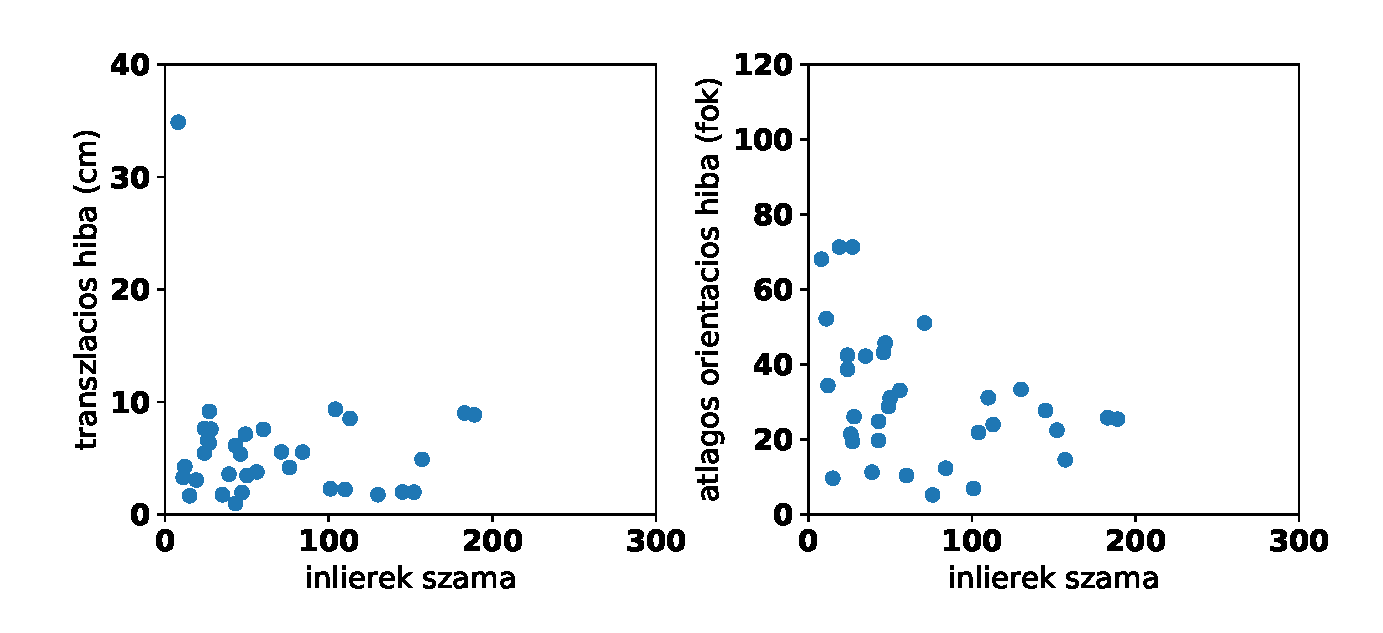
\includegraphics[width=0.9\linewidth]{chapters/results/err1.eps}
\caption{A teszt eredménye az 1. elrendezés esetében.}
\label{fig:scatter1}
\end{figure}

\begin{figure}[H]
\centering
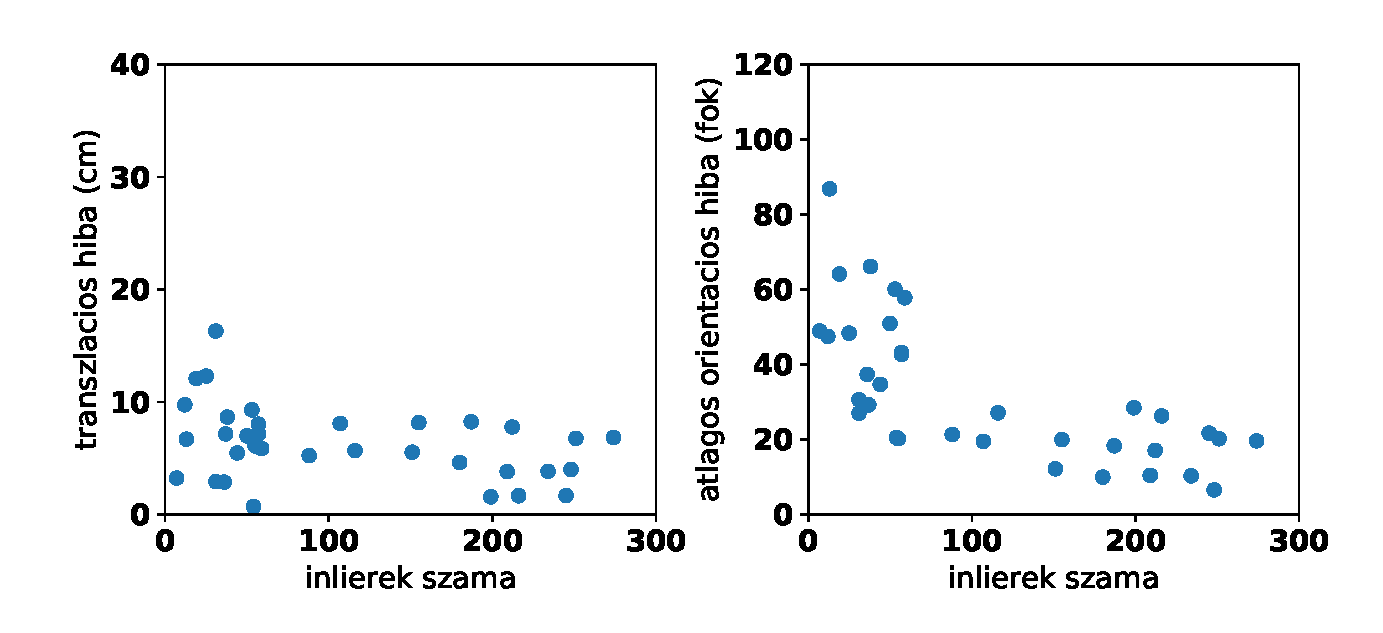
\includegraphics[width=0.9\linewidth]{chapters/results/err2.eps}
\caption{A teszt eredménye a 2. elrendezés esetében.}
\label{fig:scatter2}
\end{figure}

\begin{figure}[H]
\centering
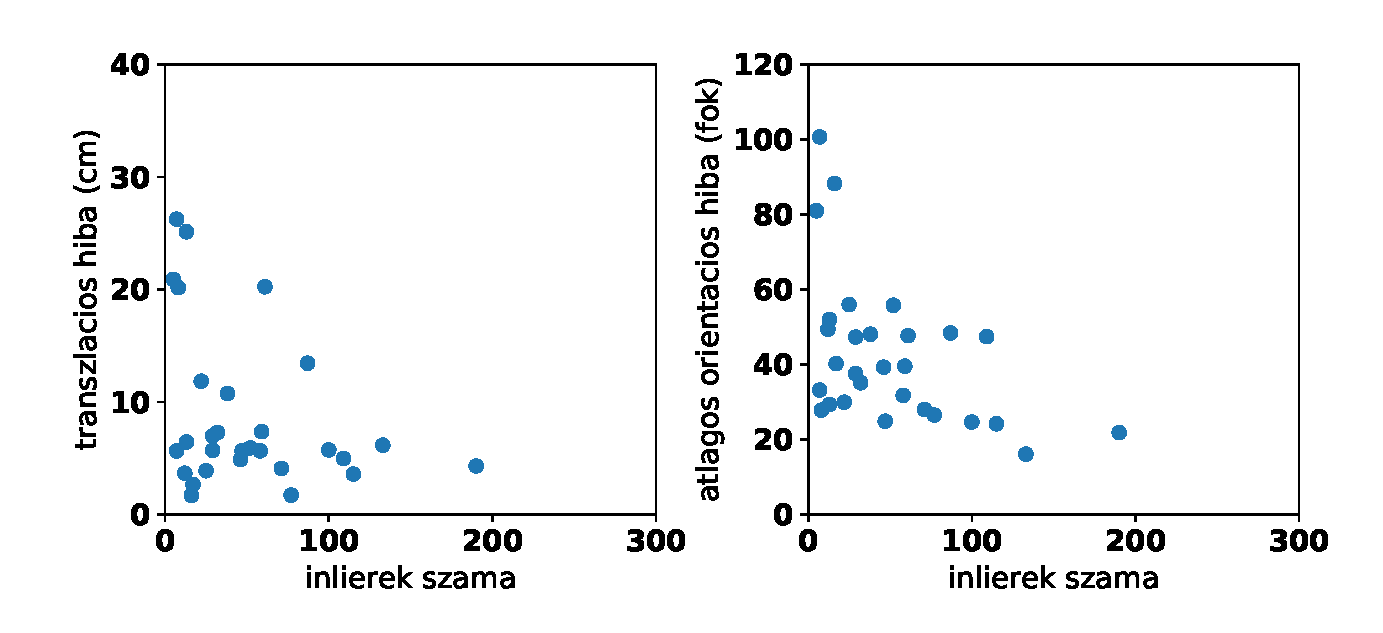
\includegraphics[width=0.9\linewidth]{chapters/results/err3.eps}
\caption{A teszt eredménye a 3. elrendezés esetében.}
\label{fig:scatter3}
\end{figure}
\chapter{Értékelés, továbbfejlesztési lehetőségek}

A tesztek eredményein látszik, hogy a program viselkedése kevéssé robusztus, ugyanarra az elrendezésre nem tud reprodukálható eredményt mutatni. A \ref{fig:scatter1}, \ref{fig:scatter2} és \ref{fig:scatter3} ábrák alapján azt lehet mondani, hogy az inlierek számának növekedésével a hiba konzisztenssé válik, de a tárgy megfogásához még mindig közel sem elég kicsi.

A hibáknak több oka is lehet. Mind a kéz-szem kalibrációnál, mind a 3D renkonstrukciónál problémát okoz, hogy a kamera látószöge és a robot munkatere kicsi. Nagyobb látószögű kamerát nem lehet használni, mert annak a torzítása is nagyobb. Nagyobb munkaterű robottal lehet ezen a hibán javítani.

Probléma lehet a kalibráló objektum minősége is. Az általam használt sakktáblamintázat hagyományos nyomtatópapírra készült, és a tesztek során akaratlanul is meggyűrődött, így a sarkai elmozdultak a feltételezett helyükről. Egy nehezebben deformálódó, pontosabb kalibráló objektum használata sokat lendíthetne a pontosság növelésén.

A kamerát technikai okokból nem tudtam a legnagyobb felbontásán használni, ez lehet, hogy segítene több kulcspontot detektálni a tárgyon és több párosítást használni. Természetesen ez valószínűleg a futásidő rovására menne. További probléma lehet még, hogy a labor megvilágítása nem kifejezetten erős, a képek zajosak, ez is zavarhatja a kulcspontpárosítást.
%%----------------------------------------------------------------------------
\chapter{\LaTeX-eszközök}\label{sect:LatexTools}
%----------------------------------------------------------------------------
\section{A szerkesztéshez használatos, Windows alapú eszközök}
%----------------------------------------------------------------------------
Ez a sablon Windows operációs rendszer alatt készült TeXnicCenter 1 Beta 7.01 szerkesztõvel. A TeXnicCenter egy \LaTeX-szerkesztõprogram számtalan hasznos -- és ráadásul jól működõ -- szolgáltatással (\figref{TexnicCenter} ábra). A szoftver ingyenesen letölthetõ a\\\url{http://www.texniccenter.org/} címrõl.

\begin{figure}[!ht]
\centering
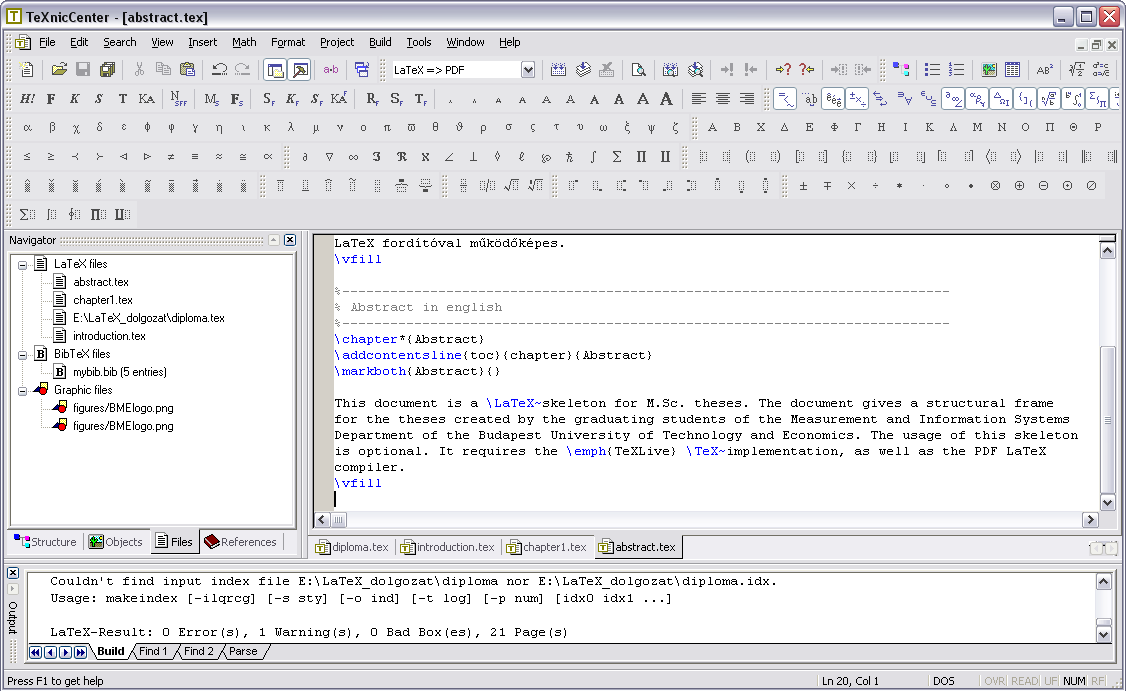
\includegraphics[width=150mm, keepaspectratio]{figures/TeXnicCenter.png}
\caption{A TeXnicCenter Windows alapú \LaTeX-szerkesztõ.} 
\label{fig:TexnicCenter}
\end{figure}

Egy másik használható Windows alapú szerkesztõprogram a LEd (LaTeX Editor,\\\url{http://www.latexeditor.org/}), a TeXnicCenter azonban stabilabb, gyorsabb, és jobban használható.

%----------------------------------------------------------------------------
\section{A dokumentum lefordítása Windows alatt}
%----------------------------------------------------------------------------
A TeXnicCenter és a LEd kizárólag szerkesztõprogram (bár az utóbbiban DVI-nézegető is van), így a dokumentum fordításához szükséges eszközöket nem tartalmazza. Windows alatt alapvetően két lehetőség közül érdemes választani: MiKTeX (\url{http://miktex.org/}) és TeXLive (\url{http://www.tug.org/texlive/}) programcsomag. Az utóbbi működik Mac OS X, GNU/Linux alatt és Unix-származékokon is. A MiKTeX egy alapcsomag telepítése után mindig letölti a használt funkciókhoz szükséges, de lokálisan hiányzó \TeX-csomagokat, míg a TeXLive DVD ISO verzióban férhető hozzá. Ez a dokumentum TeXLive 2008 programcsomag segítségével fordult, amelynek DVD ISO verziója a megadott oldalról letölthető. A sablon lefordításához a disztribúcióban szereplő \verb+magyar.ldf+ fájlt a \verb+http://www.math.bme.hu/latex/+ változatra kell cserélni, vagy az utóbbi változatot be kell másolni a projekt-könyvtárba (ahogy ezt meg is tettük a sablonban) különben anomáliák tapasztalhatók a dokumentumban (pl. az ábra- és táblázat-aláírások formátuma nem a beállított lesz, vagy bizonyos oldalakon megjelenik alapértelmezésben egy fejléc). A TeXLive 2008-at még nem kell külön telepíteni a gépre, elegendő DVD-ről (vagy az ISO fájlból közvetlenül, pl. DaemonTools-szal) használni. 

A \TeX-eszközöket tartalmazó programcsomag binárisainak elérési útját minden esetben be kell állítani a szerkesztőprogramban, például TeXnicCenter esetén legegyszerűbben a \verb+Build / Define output profiles...+ menüponttal előhívott dialógusablakban a \verb+Wizard...+ gombra kattintva tehetjük ezt meg.

A PDF-\LaTeX~használata esetén a generált dokumentum közvetlenül PDF-formátumban áll rendelkezésre. Amennyiben a PDF-fájl egy PDF-nézőben (pl. Adobe Acrobat Reader vagy Foxit PDF Reader) meg van nyitva, akkor a fájlleírót a PDF-néző program tipikusan lefoglalja. Ilyen esetben a dokumentum újrafordítása hibaüzenettel kilép. Ha bezárjuk és újra megnyitjuk a PDF dokumentumot, akkor pedig a PDF-nézők többsége az első oldalon nyitja meg a dokumentumot, nem a legutóbb olvasott oldalon. Ezzel szemben például az egyszerű és ingyenes \textcolor{blue}{Sumatra PDF} nevű program képes arra, hogy a megnyitott dokumentum megváltozását detektálja, és frissítse a nézetet az aktuális oldal megtartásával.

%----------------------------------------------------------------------------
\section{Eszközök Linuxhoz}
%----------------------------------------------------------------------------
Linux operációs rendszer alatt is rengeteg szerkesztőprogram van, pl. a KDE alapú Kile jól használható. Ez ingyenesen letölthető, vagy éppenséggel az adott Linux-disztribúció eleve tartalmazza, ahogyan a dokumentum fordításához szükséges csomagokat is. Az Ubuntu Linux disztribúciók alatt például legtöbbször a \verb+texlive-base+ csomag telepítésével használhatók a \LaTeX-eszközök.

%%----------------------------------------------------------------------------
\chapter{A dolgozat formai kivitele}
%----------------------------------------------------------------------------
Az itt található információk egy része a BME VIK Hallgatói Képviselet által készített ,,Utolsó félév a villanykaron'' c. munkából lett kis változtatásokkal átemelve. Az eredeti dokumentum az alábbi linken érhetõ el: \url{http://vik-hk.bme.hu/diplomafelev-howto-2009}.

%----------------------------------------------------------------------------
\section{A dolgozat kimérete}
%----------------------------------------------------------------------------
A minimális 50, az optimális kiméret 60-70 oldal (függelékkel együtt). A bírálók és a záróvizsga bizottság sem szereti kifejezetten a túl hosszú dolgozatokat, így a bruttó 90 oldalt már nem érdemes túlszárnyalni. Egyébként függetlenül a dolgozat kiméretétõl, ha a dolgozat nem érdekfeszítõ, akkor az olvasó már az elején a végét fogja várni. Érdemes zárt, önmagában is érthetõ mûvet alkotni.

%----------------------------------------------------------------------------
\section{A dolgozat nyelve}
%----------------------------------------------------------------------------
Mivel Magyarországon a hivatalos nyelv a magyar, ezért alapértelmezésben magyarul kell megírni a dolgozatot. Aki külföldi posztgraduális képzésben akar részt venni, nemzetközi szintû tudományos kutatást szeretne végezni, vagy multinacionális cégnél akar elhelyezkedni, annak célszerû angolul megírnia diplomadolgozatát. Mielõtt a hallgató az angol nyelvû verzió mellett dönt, erõsen ajánlott mérlegelni, hogy ez mennyi többletmunkát fog a hallgatónak jelenteni fogalmazás és nyelvhelyesség terén, valamint - nem utolsó sorban - hogy ez mennyi többletmunkát fog jelenteni a konzulens, illetve bíráló számára. Egy nehezen olvasható, netalán érthetetlen szöveg teher minden játékos számára.

%----------------------------------------------------------------------------
\section{A dokumentum nyomdatechnikai kivitele}
%----------------------------------------------------------------------------
A dolgozatot A4-es fehér lapra nyomtatva, 2,5 centiméteres margóval (+1~cm kötésbeni), 11-12 pontos betûmérettel, talpas betûtípussal és másfeles sorközzel célszerû elkészíteni.



%%----------------------------------------------------------------------------
\chapter*{Köszönetnyilvánítás}\addcontentsline{toc}{chapter}{Köszönetnyilvánítás}
%----------------------------------------------------------------------------

Ez nem kötelezõ, akár törölhetõ is. Ha a szerzõ szükségét érzi, itt lehet köszönetet nyilvánítani azoknak, akik hozzájárultak munkájukkal ahhoz, hogy a hallgató a szakdolgozatban vagy diplomamunkában leírt feladatokat sikeresen elvégezze. A konzulensnek való köszönetnyilvánítás sem kötelezõ, a konzulensnek hivatalosan is dolga, hogy a hallgatót konzultálja.

%\listoffigures\addcontentsline{toc}{chapter}{Ábrák jegyzéke}
%\listoftables\addcontentsline{toc}{chapter}{Táblázatok jegyzéke}

%

\chapter*{Ábrák forrásai}
(\ref{fig:pinhole}). Ábra: A pinhole-kameramodell.\\
Forrás: \url{http://openmvg.readthedocs.io/en/latest/openMVG/cameras/cameras/}

(\ref{fig:ransac}). Ábra: A RANSAC algoritmus és a legkisebb négyzetek módszerének összehasonlítása. \\
Forrás: \url{http://scikit-learn.org/stable/auto_examples/linear_model/plot_ransac.html}

\bibliography{mybib}
\addcontentsline{toc}{chapter}{Irodalomjegyzék}
\bibliographystyle{plain}

%%----------------------------------------------------------------------------
\appendix
%----------------------------------------------------------------------------
\chapter*{Függelék}\addcontentsline{toc}{chapter}{Függelék}
\setcounter{chapter}{6}  % a fofejezet-szamlalo az angol ABC 6. betuje (F) lesz
\setcounter{equation}{0} % a fofejezet-szamlalo az angol ABC 6. betuje (F) lesz
\numberwithin{equation}{section}
\numberwithin{figure}{section}
\numberwithin{lstlisting}{section}
%\numberwithin{tabular}{section}

%----------------------------------------------------------------------------
\section{A TeXnicCenter felülete}
%----------------------------------------------------------------------------
\begin{figure}[!ht]
\centering
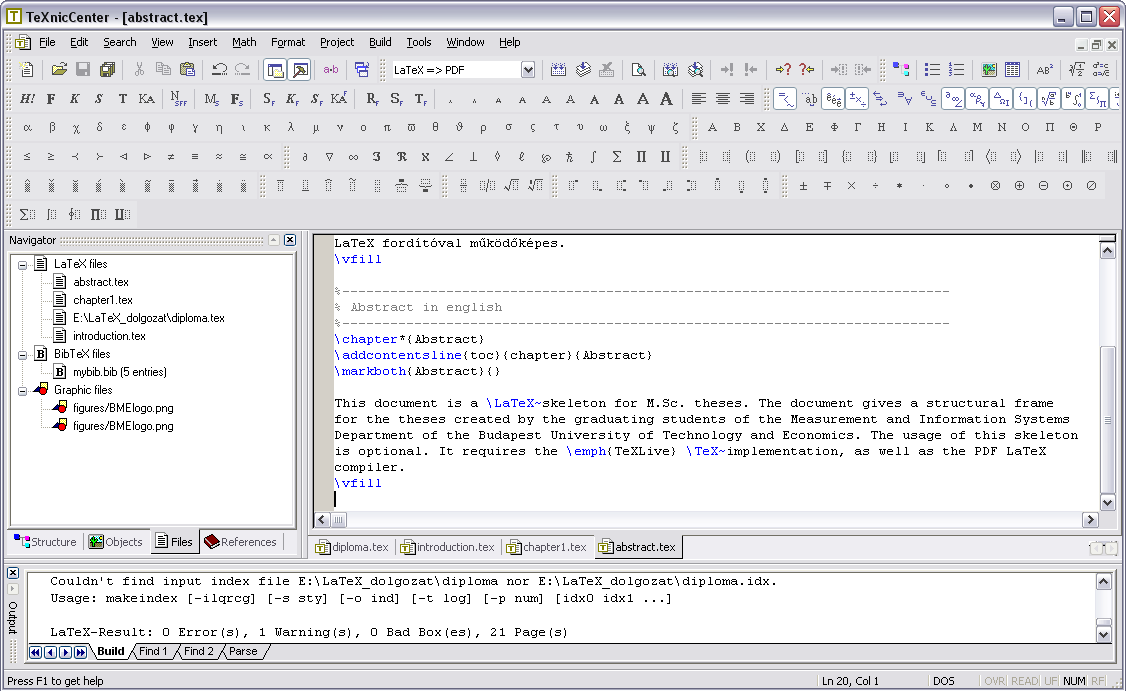
\includegraphics[width=150mm, keepaspectratio]{figures/TeXnicCenter.png}
\caption{A TeXnicCenter Windows alapú \LaTeX-szerkesztõ.} 
\end{figure}

%----------------------------------------------------------------------------
\clearpage\section{Válasz az ,,Élet, a világmindenség, meg minden'' kérdésére}
%----------------------------------------------------------------------------
A Pitagorasz-tételbõl levezetve
\begin{align}
c^2=a^2+b^2=42.
\end{align}
A Faraday-indukciós törvénybõl levezetve
\begin{align}
\rot E=-\frac{dB}{dt}\hspace{1cm}\longrightarrow \hspace{1cm}
U_i=\oint\limits_\mathbf{L}{\mathbf{E}\mathbf{dl}}=-\frac{d}{dt}\int\limits_A{\mathbf{B}\mathbf{da}}=42.
\end{align}







\label{page:last}
\end{document}
